\chapter{Application of Machine Learning Algorithms}
\label{chap:four}

\section{Repository and Environment Structure}
\section{Data Exploration}
This section is focused on exploration of the analyzed loan dataset, particularly on dataset description, distribution analysis and association analysis, in order to infer potential valuable insights and hypotheses which can be used in the preprocessing or modelling part.

\subsection{Dataset Description}
The analyzed dataset pertains to the HMEQ dataset which contains loan application information and default status of 5,960 US home equity loans. Such dataset was acquired from Credit Risk Analytics.

As can be seen in \autoref{tab:dataset}, the dataset contains 12 columns, 11 features and 1 target variable \texttt{BAD} indicating whether the loan was in default (\texttt{1}) or not (\texttt{0}). 
Amongst the 11 features, there are 9 numeric features and 2 categorical features, namely \texttt{REASON} which contains 2 categories - Debt consolidation (\texttt{DebtCon}) and Home improvement (\texttt{HomeImp}), and \texttt{JOB} which fontains following categories - Administration (\texttt{Offce}), Sales, Manager (\texttt{Mgr}), Professional Executive (\texttt{ProfExe}), Self-employed (\texttt{Self}), and Other.


\begin{table}[H]
    \small
    \setlength{\tabcolsep}{8pt}
    \renewcommand{\arraystretch}{1.3}
    \begin{center}
        \caption[Dataset columns]{Dataset columns}\label{tab:dataset}
    \begin{tabular}{@{} l p{8cm} l @{}}
    \toprule
    \textbf{Columns} & \textbf{Description} & \textbf{Data type}\\
    \midrule
    BAD & Default status & Boolean \\
    \hline
    LOAN & Requested loan amount & numeric \\
    \hline
    MORTDUE & Loan amount due on existing mortgage & numeric \\
    \hline
    VALUE & Value of current underlying collateral property & numeric \\
    \hline
    REASON & Reason of loan application & categorical \\
    \hline
    JOB & Job occupancy category & categorical \\
    \hline
    YOJ & Years of employment at present job & numeric \\
    \hline
    DEROG & Number of derogatory public reports & numeric \\
    \hline
    DELINQ & Number of delinquent credit lines & numeric \\
    \hline
    CLAGE & Age of the oldest credit line in months & numeric \\
    \hline
    NINQ & Number of recent credit inquiries & numeric \\
    \hline
    CLNO & Number of credit lines & numeric \\
    \hline
    DEBTINC & Debt-to-income ratio & numeric \\
    \bottomrule
    \end{tabular}
    \end{center}
    \begin{center} % Center the source
    \source{\url{http://www.creditriskanalytics.net/datasets-private2.html}}
    \end{center}
\end{table}


\subsection{Distribution Analysis}
In this subsection, we inspect the distribution of our variables, including the target variable and the features.
Such distribution inspection may help us to identify potential outliers, missing values, and other potential issues with the dataset.

\subsubsection{Default Distribution}

Regarding the the target variable distribution, from the \autoref{fig:defaultdist} we can observe that the default status distribution is heavily imbalanced, as most of the loans have not defaulted yet.
Particularly, 80.05\% of the observations have been labelled as non-default (4,771 observations) and 19.95\% observations labelled as default (1,189 observations).
This may cause problems in the modelling part, as the model may be biased towards the majority class, i.e., the non-default class. Such imbalanced class issue will be further treated in \autoref{subsec:data-split-ADASYN}.

\begin{figure}[H]
    \centering
    \caption{Default status distribution}
    \label{fig:defaultdist}
    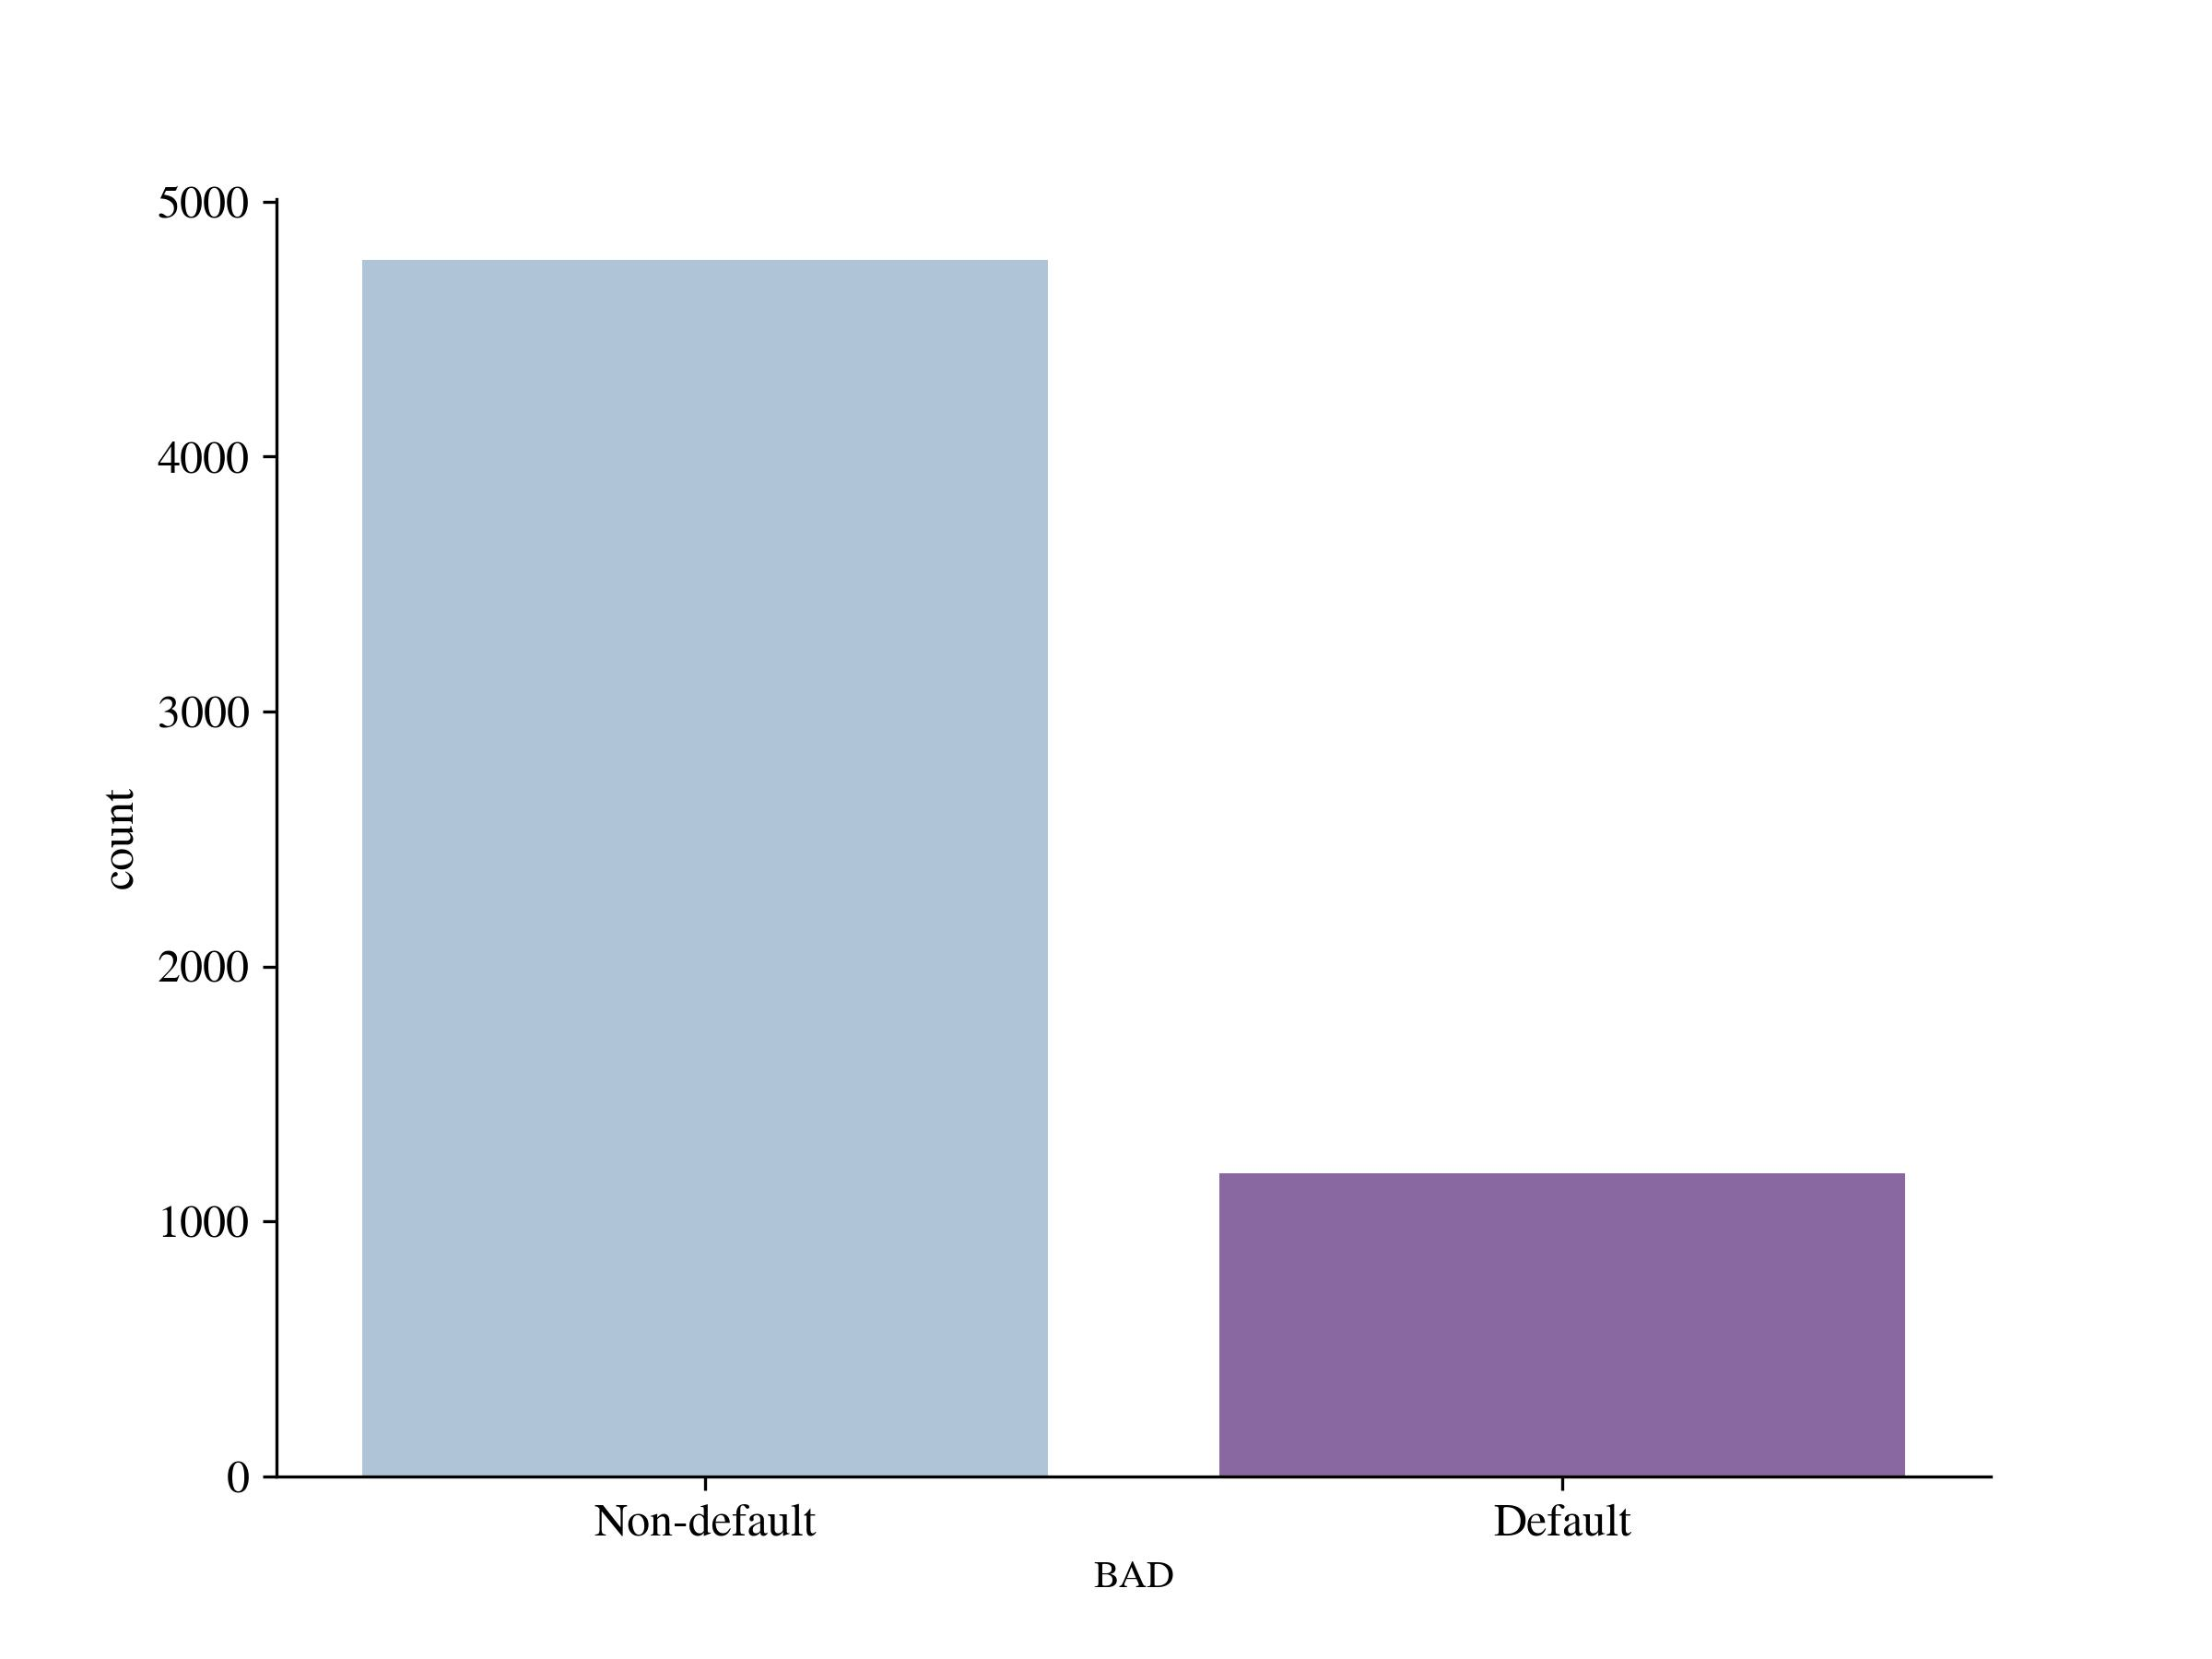
\includegraphics[width=150mm]{Figures/Default_Distribution.jpg}\vspace{-1em}
\centering{\begin{source}Author's results in Python.\end{source}}\vspace{-1em}
\end{figure}

\subsubsection{Numeric Features' Distribution}
\label{subsubsec:numdist}

With regards to the numeric features, most of the features are positively skewed containing outliers as can be seen in \autoref{fig:boxfeat}, which depicts conditional distribution of numeric features on the default status visualized using boxplots.

All the outliers appear to be valid, i.e., they have not occurred due to data entry errors.
This can be attributed to the fact that all the numeric features are non--negative, thus it is not possible to have negative number of years at present job, negative number of delinquent credit lines, etc. 
Furthermore, the maximum values of given features are not unrealistically high, which further confirms the validity of the outliers.
Nevertheless, the outliers need to be treated since they can biased model's weights or coefficients (in case of logistic regression or neural networks), jeopardize distance calculation (in case of KNN) or in general, they can affect the position and orientation of the decision boundary -- all the reasonings can lead to the model's overfitting and inaccurate and biased predictions.
The outliers' treatment is further described in \autoref{subsec:prep-optbinning}.

With respect to the target variable, we can observe some differences in the distribution shapes of \texttt{DEROG} and \texttt{DELINQ}, which are less skewed and have lower dispersion for non--default cases compared to the default cases.
Since both features indicates a negative information about the delinquency, it is expected that the higher value is, the more likely the loan will end in default.
Referring to the feature \texttt{DEBTINC}, it does not have any extreme values for non--default cases, but it has some extreme values for default cases. We can infer that if the debt--to--income ratio is too high, hence applicant's income is not sufficient to cover his debt, the loan is more likely to end in default.
The assocation between the default status and the numeric features is further investigated in \autoref{subsubsec:target-num-ass}.

\begin{figure}[H]
    \centering
    \caption{Conditional distribution of numeric features}\vspace{0.5em}
    \label{fig:boxfeat}
    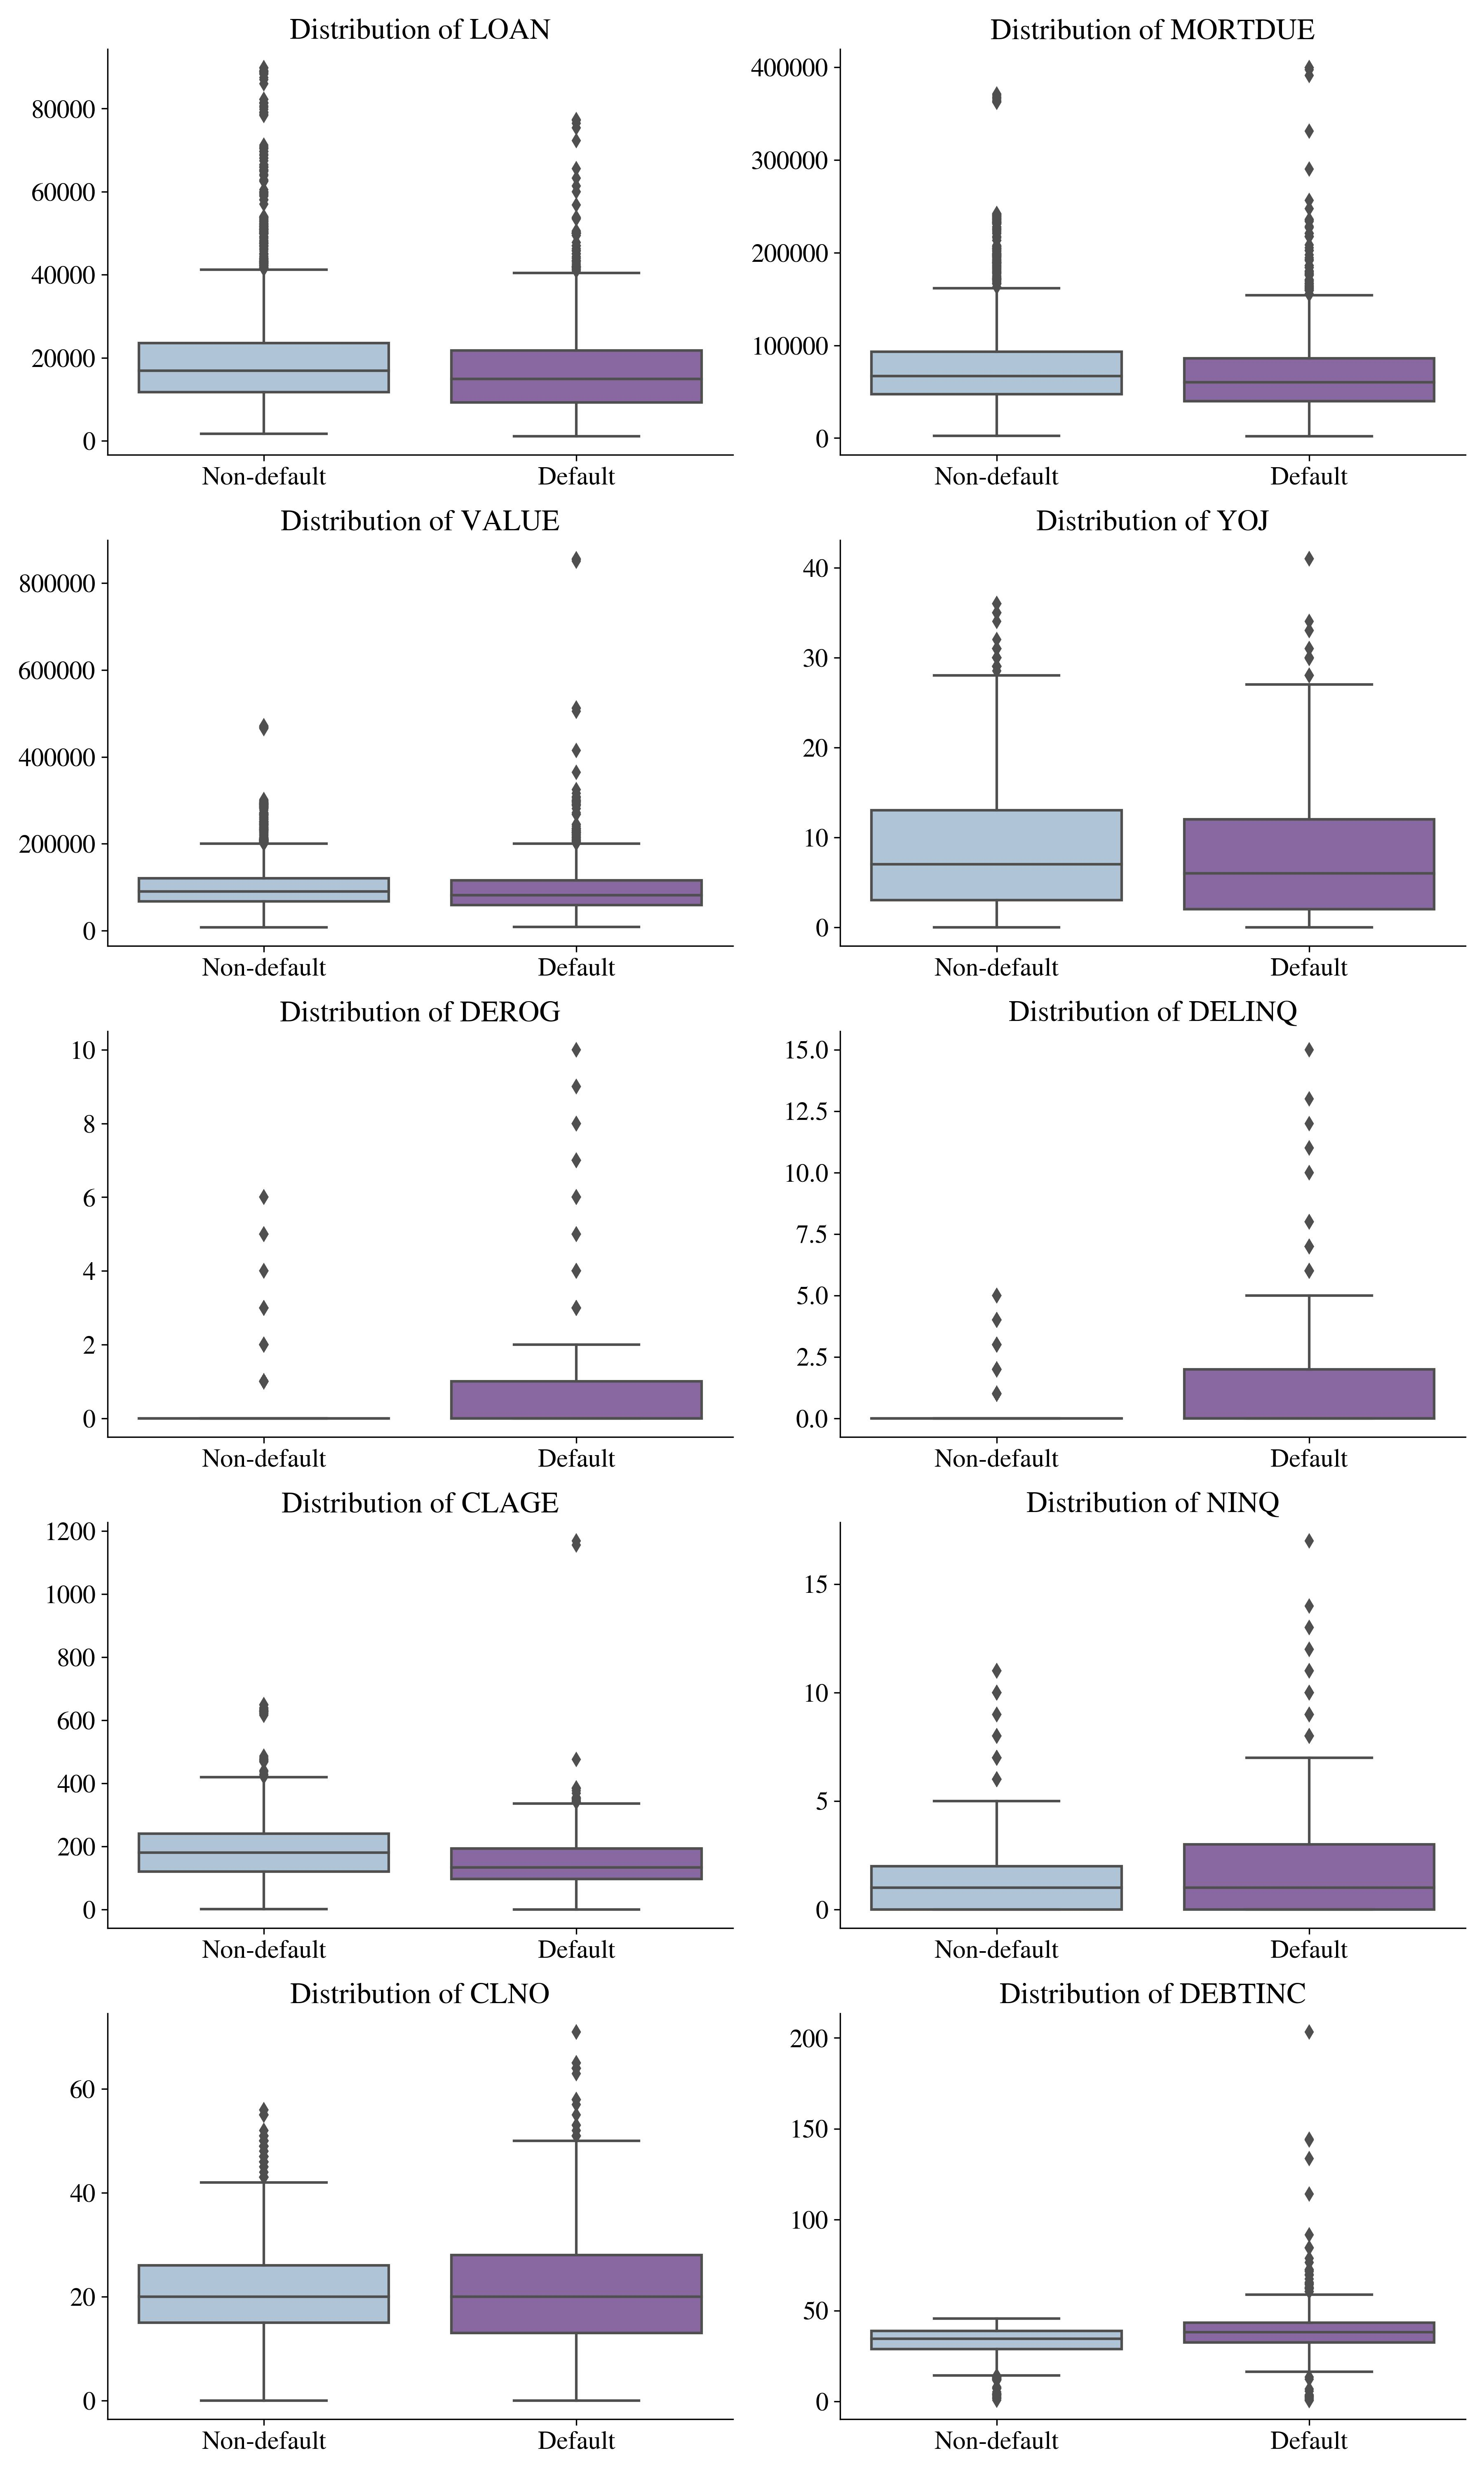
\includegraphics[width=140mm]{Figures/Continuous_Features_Distribution_Boxplots.jpg}
    \centering{\begin{source}Author's results in Python.\end{source}}\vspace{-1em}
\end{figure}

Due to the fact that the boxplots do not capture the missing values occurred in given features, it is also important to inspect the numbers and proportions of missing values in each feature, conditional on the default status.
As can be seen in \autoref{tab:nacont-table}, $n_0$ refers to the number of missing values in given feature for non-default cases, $n_1$ refers to the number of missing values in given feature for default cases.
$N_0$ and $N_1$ refer to the total number non--default cases and default cases respectively, therefore $n_0/N_0$ refers to the proportion of missing values in given feature for non-default cases, and $n_1/N_1$ refers to the proportion of missing values in given feature for default cases.

Pertaining to the feature \texttt{DEBTINC}, we can observe a significant difference in the number of missing values between the default and non-default cases. Out of all defaulted loans, 66.11 \% had missing debt--to--income ratio, whereas only 10.08 \% out of all non-defaulted loans had missing debt--to--income ratio.
Therefore, there could be a strong association between the missing debt--to--income ratio and the default.

Similarly, the table depicts a significant difference with respect to \texttt{VALUE} as 0.15 \% had missing collateral property value out of all non--defaulted loan, and 8.92 \% defaulted loans had missing collateral property value.
It can be inferred that loan applicants who withhold information on their collateral property value or debt-to-income ratio are more likely to default on their loans.
This may be due to negative information that they are trying to conceal, such as an excessively high debt or low income, or a low collateral property value.
Such associations are further investigated in \autoref{subsubsec:target-na-ass}.


\begin{table}[H]
    \small
    \setlength{\tabcolsep}{8pt}
    \renewcommand{\arraystretch}{1.3}
 % define a new column type 'L' for left alignment
    \newcolumntype{R}[1]{>{\raggedleft\arraybackslash}p{#1}} % define a new column type 'R' for right alignment
    \begin{center}
        \caption[Numeric features NA's table]{Numeric features NA's table}\label{tab:nacont-table}
        \begin{tabular}{l R{1cm}R{1cm}|R{1.5cm}R{1.5cm}}
            \toprule
            \textbf{Feature} & \textbf{$n_0$} & \textbf{$n_1$} & \textbf{$n_0/N_0$} & \textbf{$n_1/N_1$} \\
            \midrule
            \hline
            LOAN & 0 & 0 & 0 \% & 0 \% \\

            MORTDUE & 412 & 106 & 8.64 \% & 8.92 \% \\
 
            VALUE & 7 & 105 & 0.15 \% & 8.83 \% \\
   
            YOJ & 450 & 65 & 9.43 \% & 5.47 \% \\

            DEROG & 621 & 87 & 13.02 \% & 7.32 \% \\

            DELINQ & 508 & 72 & 10.65 \% & 6.06 \% \\

            CLAGE & 230 & 78 & 4.82 \% & 6.56 \% \\

            NINQ & 435 & 75 & 9.12 \% & 6.31 \% \\

            CLNO & 169 & 53 & 3.54 \% & 4.46 \% \\

            DEBTINC & 481 & 786 & 10.08 \% & 66.11 \% \\ \hline
            \bottomrule
        \end{tabular}
    \end{center}
    \begin{center}
        \source{Author's results in Python}
    \end{center}
\end{table}


\subsubsection{Categorical Features' Distribution}
\label{subsubsec:catdist}

Pertaining to the categorical features, such dataset has 2 nominal features - \texttt{REASON} and \texttt{JOB}. The following \autoref{fig:catdist} depicts the conditional distribution of categorical features on the default status visualized using barplots.
We can observe that most of the loan applicants applied for a loan because of the debt consolidation and/or their job occupancies were labelled as \texttt{Other}.

Regarding the default status, there does not seem to be a significant difference between the default and non-default cases in terms of relative distribution of \texttt{REASON}.
However, we can observe a slight difference between the default and non-default cases in terms of relative distribution of \texttt{JOB} feature. Particularly, in the categories \texttt{Office}, \texttt{ProfExe} and \texttt{N/A} there is relatively higher proportion of non--default cases than default cases. Therefore, there could be a moderate association between the \texttt{JOB} feature and the default status -- such association is further investigated in \autoref{subsubsec:target-cat-ass}.


\begin{figure}[H]
    \centering
    \caption{Conditional distribution of categorical features}\vspace{0.5em}
    \label{fig:catdist}
    \includegraphics[width=140mm]{Figures/Categorical_Features_Distribution.jpg}
    \centering{\begin{source}Author's results in Python.\end{source}}\vspace{-1em}
    \end{figure}

\subsection{Association Analysis}
In this subsection, we focus on the association analysis in order to inspect potential relationships between the variables. First, we inspect the association between the default status and the features and aftewards, we check for the association amongst the features themselves.


\subsubsection{Association between default status and numeric features}
\label{subsubsec:target-num-ass}

In order to measure an association between the target variable and the numeric features, we use Point--Biserial correlation which denotes the value of Pearson's product moment correlation between the continuous variable and dichotomous variable \citep{kornbrot2014point}. Such coefficient ranges from -1 to +1.

\begin{equation}\label{eq}
    r_{pb,X} =  \frac{\mu \left( X | Y=1 \right) -\mu \left( X | Y=0 \right)}{\sigma_{X}}\sqrt{\frac{N\left(Y=1\right) \times N\left(Y=0\right)}{N \left(N - 1 \right)}}
\end{equation}

where $\mu \left( X | Y=1 \right)$ and $\mu \left( X | Y=0 \right)$ are the means of given numeric feature $X$ conditional on the default status and non--default status, respectively, $\sigma_{X}$ is the standard deviation of given numeric feature $X$, $N\left(Y=1\right)$ and $N\left(Y=0\right)$ are the numbers of observations with default status and non--default status, respectively, and $N$ is the total number of observation within given feature $X$.


In the following \autoref{tab:pointbi}, we can observe the computed Point-Biserial coefficient for each numeric feature with respect to the default status, including its statistical significance.
As can be seen, features such as \texttt{DEROG}, \texttt{DELINQ} and \texttt{DEBTINC} are moderately and positively association with default status on 1\% statistical significance level.
Thus, we can confirm the findings from \autoref{subsubsec:numdist} regarding the positive associations of the features \texttt{DEROG}, \texttt{DELINQ} and \texttt{DEBTINC} with the default status.
It can be deemed and inferred that such features may be important predictors within modelling.

    \begin{table}[H]
        \small
        \setlength{\tabcolsep}{8pt}
        \renewcommand{\arraystretch}{1.3}
        \centering
            \caption[Point--Biserial Correlation table]{Point--Biserial Correlation table}\label{tab:pointbi}
            \begin{tabular}{@{} l r @{\hspace{1cm}} l @{}}
        \toprule
        \textbf{Feature} & \textbf{Coefficient} & \textbf{Significance}\\
        \midrule
        \hline
       
        LOAN & -0.075  & ***\\
       
        MORTDUE & -0.048  & ***\\
       
        VALUE & -0.030  & ** \\
        
        YOJ & -0.060  & *** \\
      
        DEROG & 0.276 & *** \\
     
        DELINQ & 0.354 & *** \\
        
        CLAGE & -0.170 & *** \\

        NINQ & 0.175 & *** \\

        CLNO & -0.004 & \\

        DEBTINC & 0.200 & *** \\
        \hline
        \bottomrule
        \end{tabular}
        \vspace{0.35em}

    
            \centering\footnotesize{$^{*}$: $p<0.10$, $^{**}$: $p<0.05$, $^{***}$: $p<0.01$}\vspace{0.7em}

            \centering{\begin{source}Author's results in Python.\end{source}}\vspace{-1em}

    \end{table}

ok

ok

\subsubsection{Association between default status and categorical features}
\label{subsubsec:target-cat-ass}

For measuring a relationship's strength between the dichotomous and categorical variables, we use Cramer's V which ranges from 0 to 1 and is defined as:

\begin{equation}\label{eq}
		CV_{X} = \sqrt{\frac{\chi^{2}}{N\left(k-1\right)}}
		\end{equation}

As expected based on findings in \autoref{subsubsec:catdist}, according to the following \autoref{tab:cramer-v}, the association between the default status and \texttt{REASON} is really weak as the Cramer's V is close to zero.
On the other hand, we can observe slightly stronger association of \texttt{JOB} with default status as some of its categories, namely \texttt{Office}, \texttt{ProfExe} and \texttt{N/A}, showed a higher proportion of non--default cases compared to the default cases. 
Note both \texttt{REASON}'s and \texttt{JOB}'s associations with default status are statistically significant on 1\% significance level.
Although statistical significance is important, it does not guarantee that a feature is a strong predictor of the target variable. Ultimately, the performance metrics of the model are what determine the usefulness of a feature in predicting the target variable.


        \begin{table}[H]
            \small
            \setlength{\tabcolsep}{8pt}
            \renewcommand{\arraystretch}{1.3}
            \centering
                \caption[Cramer's V Association table]{Cramer's V Association table}\label{tab:cramer-v}
                \begin{tabular}{@{} l r @{\hspace{1cm}} l @{}}
            \toprule
            \textbf{Feature} & \textbf{Coefficient} & \textbf{Significance}\\
            \midrule
            \hline
            REASON & 0.038  & ***\\
            JOB & 0.120  & ***\\
            \hline

            \bottomrule
        \end{tabular}
        \vspace{0.35em}

    
            \centering\footnotesize{$^{*}$: $p<0.10$, $^{**}$: $p<0.05$, $^{***}$: $p<0.01$}\vspace{0.7em}

            \centering{\begin{source}Author's results in Python.\end{source}}\vspace{-1em}
\end{table}


\subsubsection{Association between default status and missing values}
\label{subsubsec:target-na-ass}

Since the loan data contains missing values, it is deemed appropriate to check whether the missing values are associated with the default status as well. One way how to deal with the measurement, is to encode the feature into a binary variable where 1 indicates a missing value occurrence and 0 otherwise.

For measuring a strength of association between the two binary variables, we use Phi coefficien which is defined as:

\begin{equation}\label{eq}
    \phi_{X} = \sqrt{\frac{\chi^{2}}{n}}
    \end{equation}

In line with the finding regarding the \texttt{DEBTINC} and \texttt{VALUE} in \autoref{subsubsec:numdist}, as shown in \autoref{tab:phi-target}, we can observe a strong and statistically significant association between the missing debt--to--income and default status, respectively a moderate and statistically significant association between the missing collateral property value and the default status. Hence, we can expect such indicators will be the main drivers in a default prediction.

    \begin{table}[H]
        \small
        \setlength{\tabcolsep}{8pt}
        \renewcommand{\arraystretch}{1.3}
        \centering
            \caption[Phi Correlation Coefficient table]{Phi Correlation Coefficient table}\label{tab:phi-target}
            \begin{tabular}{@{} l r @{\hspace{1cm}} l @{}}
        \toprule
        \textbf{Feature} & \textbf{Coefficient} & \textbf{Significance}\\
        \midrule
        \hline
        LOAN & 0.000  & \\
        \hline
        MORTDUE & 0.003  & \\
        \hline
        VALUE & 0.254  & *** \\
        \hline
        REASON & 0.004 & \\
        \hline
        JOB & 0.064 & *** \\
        \hline
        YOJ & 0.056  & *** \\
        \hline
        DEROG & 0.070 & *** \\
        \hline
        DELINQ & 0.061 & *** \\
        \hline
        CLAGE & 0.030 & ** \\
        \hline
        NINQ & 0.039 & *** \\
        \hline
        CLNO & 0.018 & \\
        \hline
        DEBTINC & 0.547 & *** \\
        \bottomrule
        \end{tabular}
        \vspace{0.35em}
 
    
            \centering\footnotesize{$^{*}$: $p<0.10$, $^{**}$: $p<0.05$, $^{***}$: $p<0.01$}\vspace{0.7em}

            \centering{\begin{source}Author's results in Python.\end{source}}\vspace{-1em}
\end{table}


\subsubsection{Missing Values Association}
Furthermore, it is needed to inspect how the missing values are related to default status, but also how they are associated between themselves.
One way, how to indetify any patterns of missing data in dataset is using dendrogram which hierarchically clusters the variables based on the missing values' occurrences.
Hence it groups the variables into clusters based on the similarity of their missing value patterns ,i.e., variables with similar patterns of missingness are clustered together, while variables with dissimilar patterns of missingness are placed in separate clusters.
The dendrogram is constructed by iteratively merging the two closest clusters until all variables are in the same cluster.
The distance between the clusters at each step of the merging process is shown on the y-axis of the dendrogram, and the order in which the variables are merged is shown on the x--axis.

The following \autoref{fig:dendrogram} depicts the hierarchical clustering of the dataset's variables, excluding the default status the requested loan amount \texttt{LOAN} since these variables do not contain any missing values.
As can be seen, features \texttt{CLNO} and \texttt{CLAGE} are the most similar in terms of missing values' occurrences
Thus, most of the loan applicants, when submitting their loan application, they oftenly omit their number of credit lines (\texttt{CLNO}) as well as the age of their recent credit line (\texttt{CLAGE}).

    \begin{figure}[H]
        \centering
        \caption{Nullity dendrogram}\vspace{0.5em}
        \label{fig:dendrogram}
        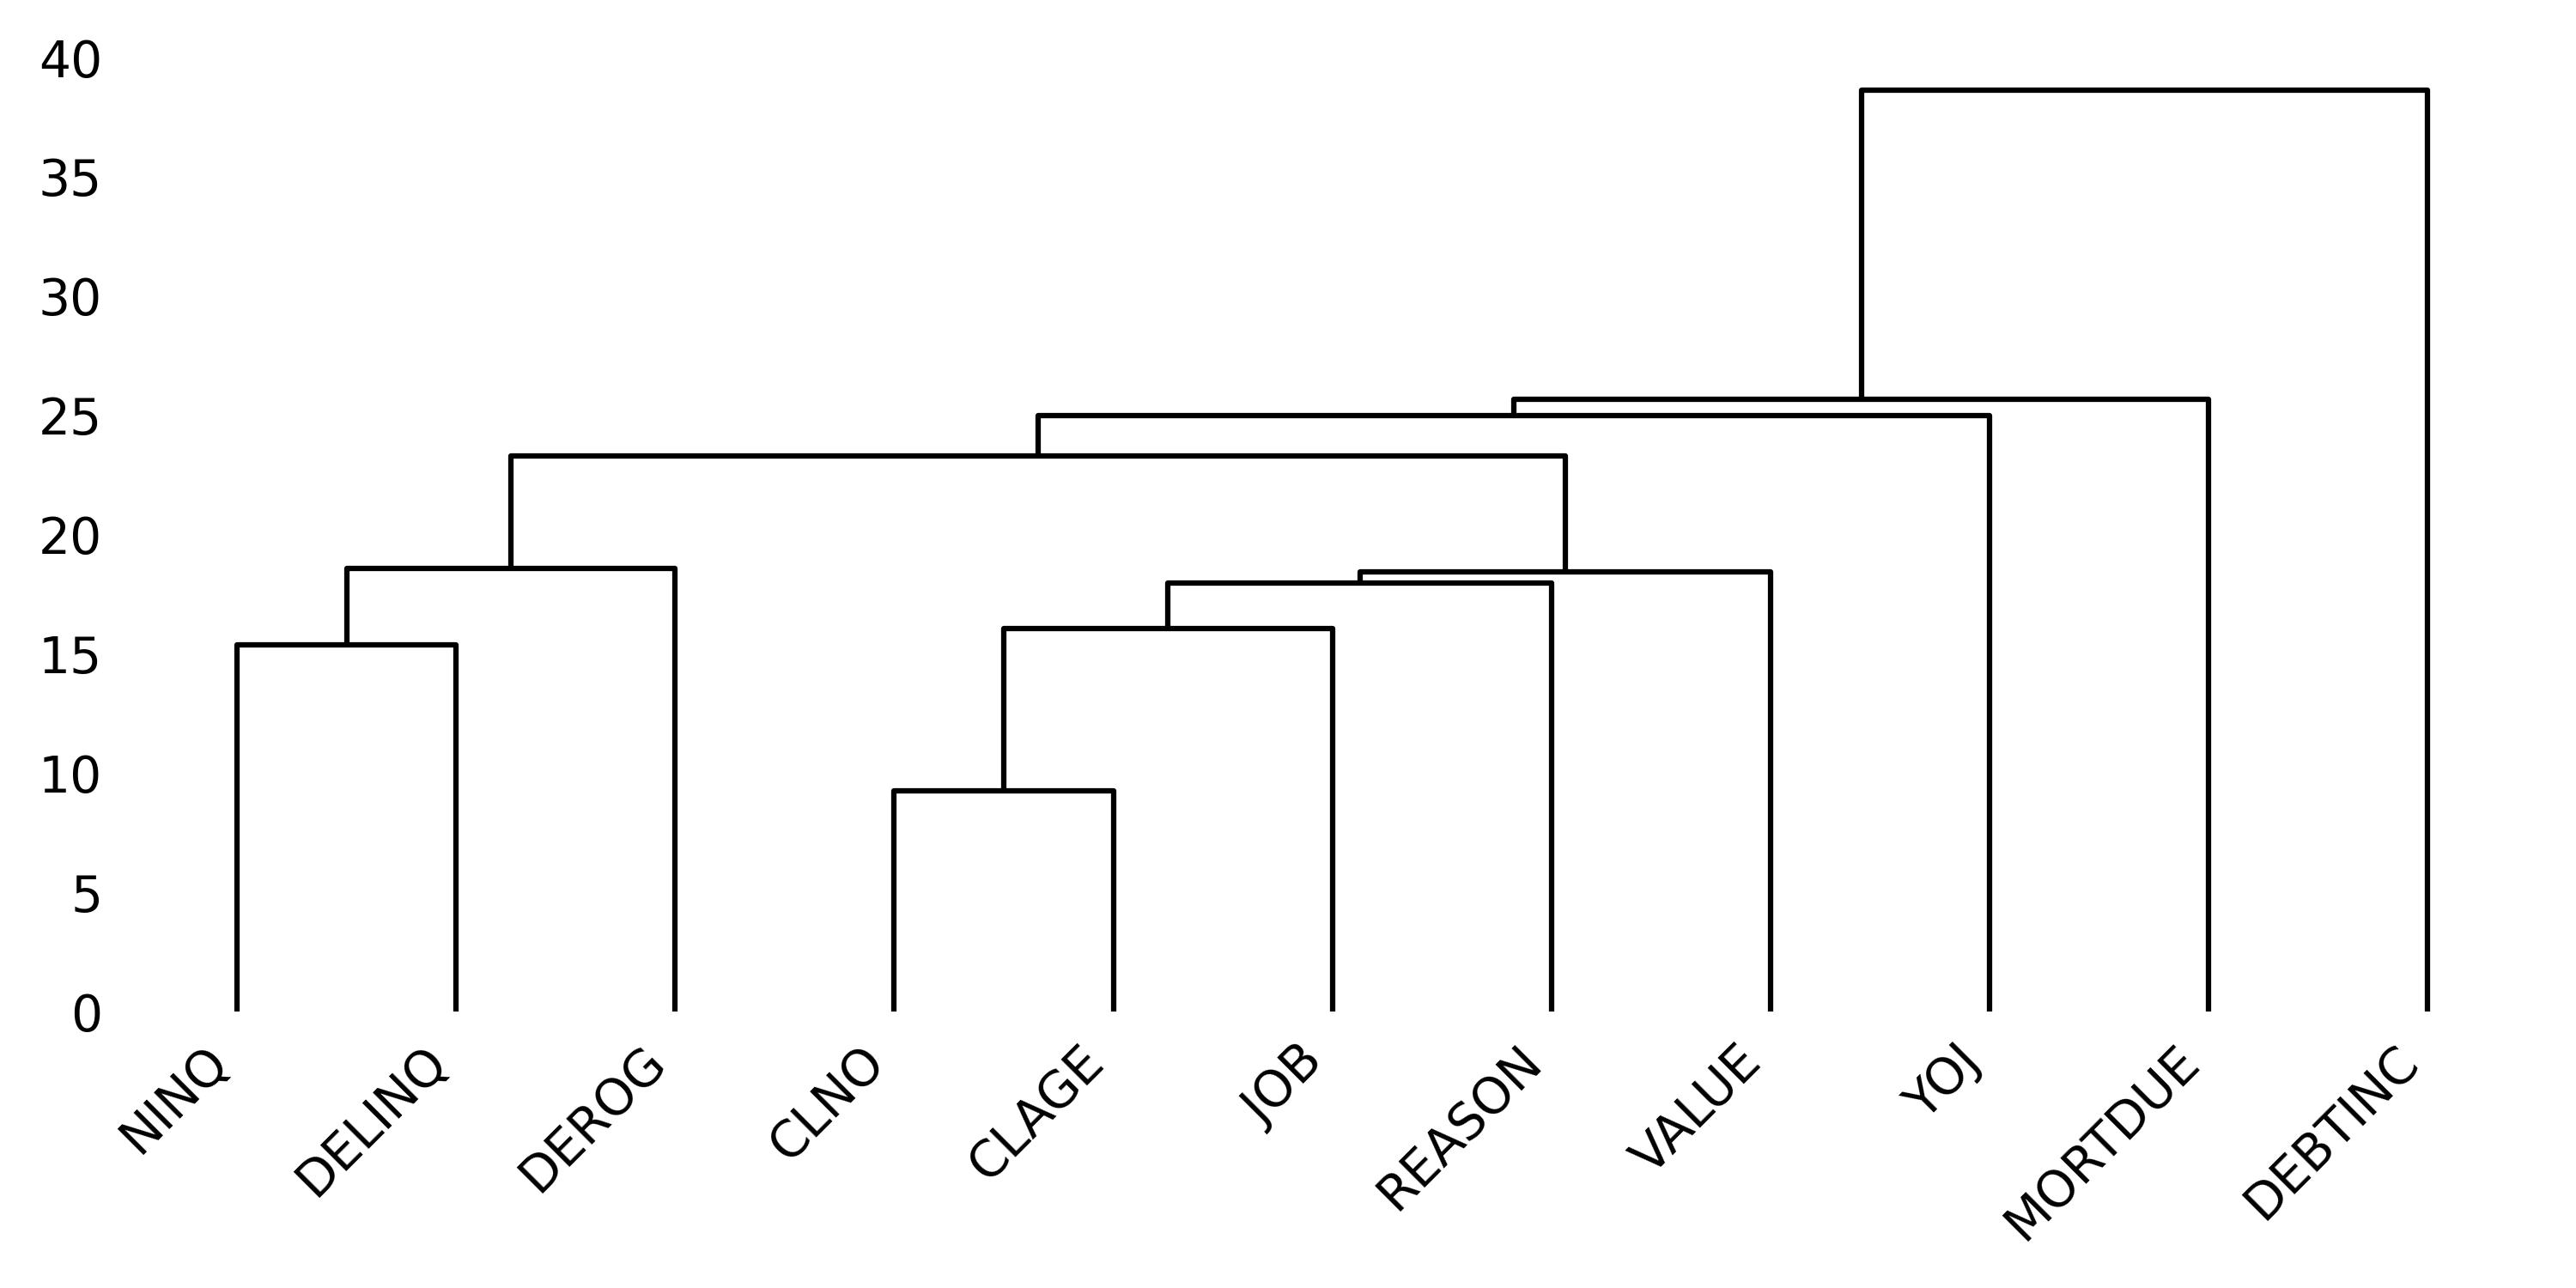
\includegraphics[width=150mm]{Figures/NA_Dendrogram.jpg}
        \centering{\begin{source}Author's results in Python.\end{source}}\vspace{-1em}
    \end{figure}
    

\subsubsection{Multicolinearity Analysis}

ADD contigency table for REASON and JOB.

To measure the correlation between the numeric features, one would use Pearson correlation coefficient. However, such measure is very sensitive to outliers and assumes normal distribution of variables as well as the linear relationship between the variables. Therefore, we use Spearman correlation coefficient instead, which is a nonparametric measure of the association between two continuous variables. It is defined as:

\begin{equation}\label{eq}
	\rho_{spearman} = 1 - \frac{6 \sum_{i=1}^{n} d_{i}^{2}}{n \left(n^{2}-1\right)}
	\end{equation}


In the \autoref{fig:spearmancorr}, we can observe a very strong correlation between the \texttt{MORTDUE} and \texttt{VALUE} features. Such multicolinearity can cause problem in predictions na model's overfitting. Therefore, a feature selection is recommended - such selection is further described in \autoref{subsec:feature-selection}.

    \begin{figure}[H]
        \centering
        \caption{Spearman Correlation Matrix}\vspace{0.5em}
        \label{fig:spearmancorr}\
        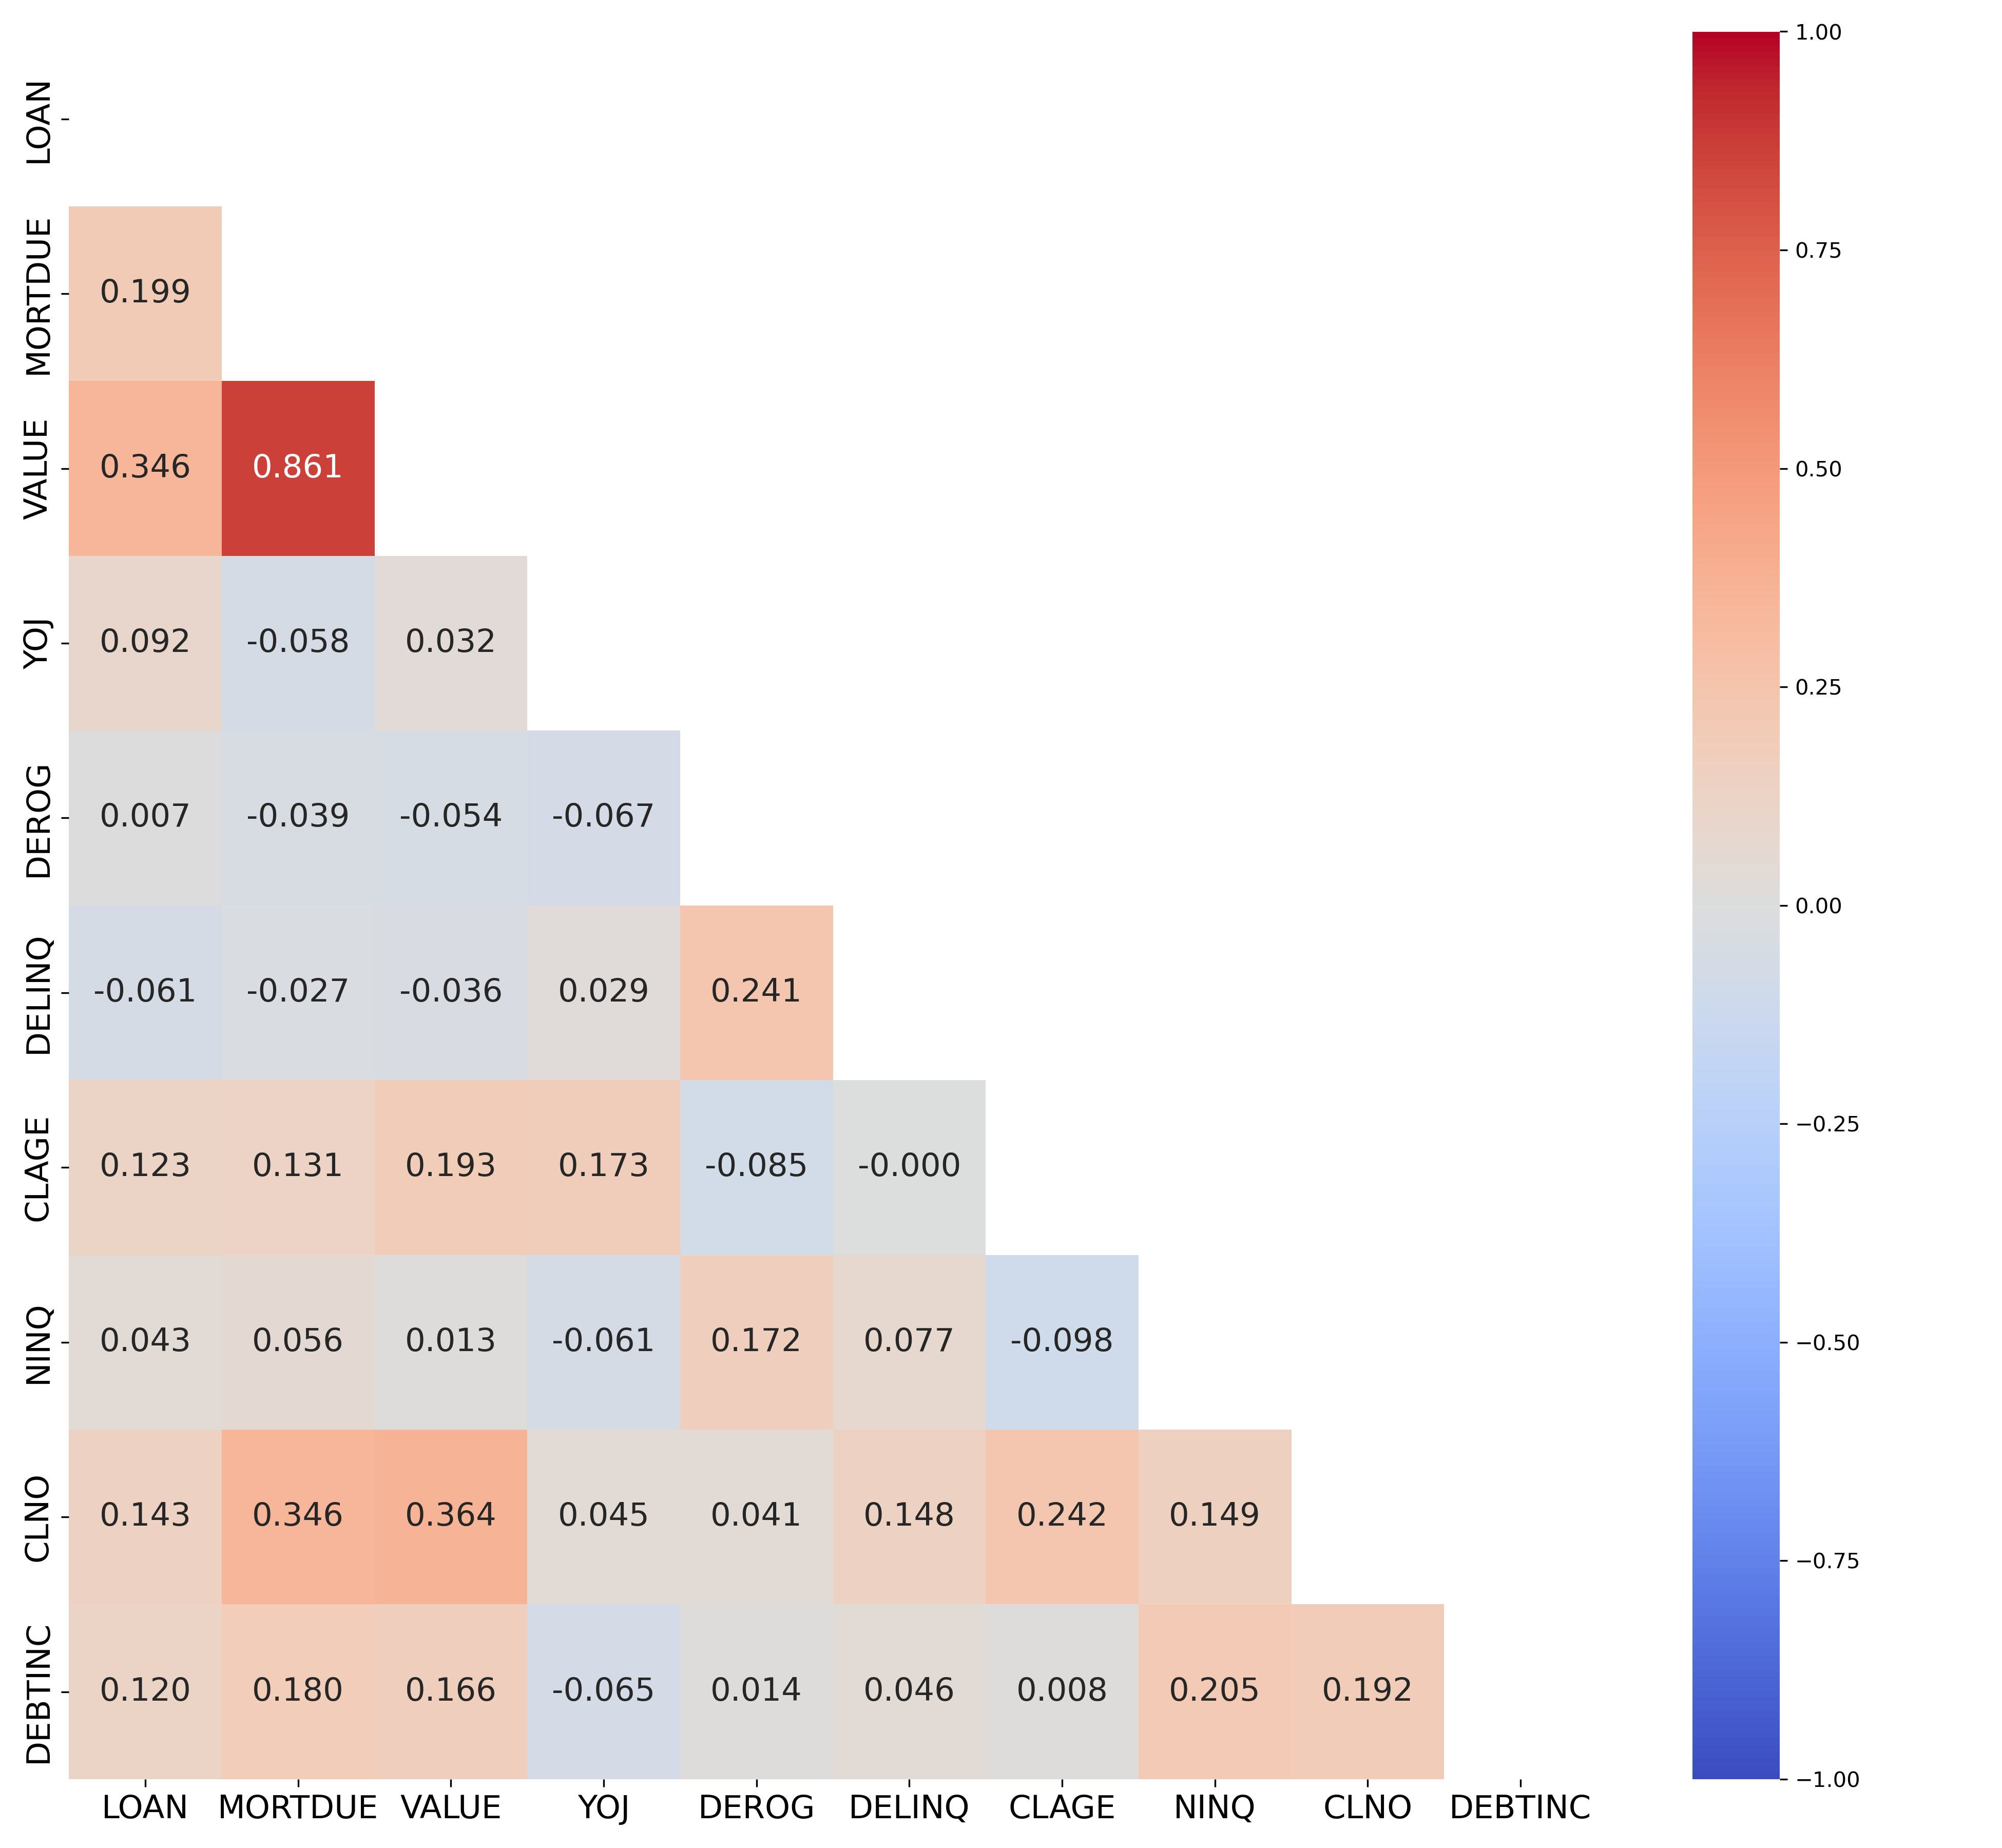
\includegraphics[width=150mm]{Figures/Spearman_Correlation_Matrix_Continuous_Features.jpg}
        \centering{\begin{source}Author's results in Python.\end{source}}\vspace{-1em}
    \end{figure}

\section{Data Preprocessing}
In this section, the process of preprocessing data is described as the crucial step in the machine learning modelling. Particularly, the following is described:
\begin{itemize}\setlength\itemsep{0em}
    \item Splitting the data
    \item oversampling,
    \item discretization,
    \item Weight--of--Evidence encoding.
\end{itemize}


\subsection{Data Split and ADASYN Oversampling}
\label{subsec:data-split-ADASYN}

In order to ensure the appropriate model training and unbiased evaluation, it is needed to split our data into sets where each sample has its own purpose. We split our data into following sets in the ratio of 70:15:15:
\begin{itemize}\setlength\itemsep{0em}
    \item Training set - such set is used for training the model, feature selection and hyperparameter tuning.
    \item Validation set - such set is used for selection of the best final model.
    \item Test set - such set is used for the final evaluation of the best final model.
\end{itemize}

It is important to split the data into separate sets so we could independently train and tuned the several models as well as choose the best features, select the best model and evaluate it on the unseen data as we ensure an avoidance of overfitting as well as the data leakage.

As already, since the default status distribution highly imbalanced, it is needed to treat such issue, otherwise the model would be biased towards the non--defaults.
Hence, the data is split into such sets using stratified split, which ensures that the default status distribution remains the same across all the sets.
Thus, when splitting the data with a stratification, the default distribution is each set is preserved, i.e., 80 \% of non--defaults and 20 \% of defaults in each set.
With a stratification, it is possible to train the model on the same population in which it is being evaluated leading to more accurate predictions \citep{igareta2021strat}.

Despite the stratification, it does not have to be sufficient when dealing with imbalanced class.
One approach is to use undersampling which removes the instances with majority class.
However, this is not deemed appropriate since our data sample size is relatively small and we would lose a lot of information by removing such instances.
Other approach is to use random oversampling, which randomly duplicates the instances of minority class in such way that the target distribution is then balanced.
Although, this is not deemed appropriate as well since as it could lead to the overfitting as the model would just memorize the duplicated instances and would not be able to generalize well on the unseen data.

Instead, ADASYN (Adaptive Synthetic Sampling) is used, which is an oversampling technique that generates synthetic instances of the minority class based on the nearest neighbors of the minority class instances.
Compared to SMOTE (Synthetic Minority Oversampling Technique), ADASYN is more effective as it uses density distribution of each minority instance which generates more synthetic samples in regions where the density of the minority class is lower and fewer synthetic instances in regions where the density is higher.
In other words, ADASYN focuses on difficult--to--learn minority instances, i.e., instances having lower density, therefore it generates more synthetic instances for such instances \citep{adasynhaibo}. Thereby, it makes easier for the machine learning model to learn the decision boundary between the minority and majority classes and boost the model's performance. 

It is important to emphasize, that the oversampling has to be performed on the training set only after the split and not before the split or on validation or test sets. Otherwise it would lead to data leakage and biased evaluation of the model.
In the following \autoref{tab:split}, we can observe some split information regarding the individual sets. As can be seen,  either test, validation and training sets (before oversampling) have the same default distribution which is desired thanks to the stratification. The table also depicts the information about the training set after performed ADASYN oversampling, where the default distribution is balanced. 

\begin{table}[H]
    \small
    \setlength{\tabcolsep}{8pt}
    \renewcommand{\arraystretch}{1.3}
    \centering
        \caption[WoE distribution]{WoE distribution}\label{tab:split}
        \begin{tabular}{lrrr}
    \toprule
    \textbf{Set} & \textbf{\# instances} & \textbf{\% defaults} & \textbf{\% non--defaults}\\
    \midrule
    \hline
    Training & 4,171  & 19.95 \% & 80.05 \% \\
    Training (oversampled) & 6,437 &  48.13 \% & 51.87 \% \\

    Validation & 895 &  20.00 \% & 80.00 \% \\

    Test & 894 &  20.00 \% & 80.00 \% \\
    \bottomrule
    \end{tabular}
    \vspace{0.7em}

    \centering{\begin{source}Author's results in Python.\end{source}}\vspace{-1em}
\end{table}

In Python, the data are split and oversampled using a custom function \lstinline{data_split()} which first splits the data into training, validation and test sets using \lstinline{train_test_split()} function with a stratification from \lstinline{scikit-klearn} module. Then, the training set is oversampled using \lstinline{ADASYN()} class with 5 nearest neighbors and Euclidean distance from \lstinline{imblearn} module. 

However, the \lstinline{imblearn}'s \lstinline{ADASYN()} class cannot handle either missing values or categorical variables. Therefore, the approach in order to deal with such obstacle is following:
\begin{enumerate}\setlength\itemsep{0em}
    \item Separate the categorical and numeric features;
    \item Impute the missing values with arbitrary values:
    \begin{itemize}\setlength\itemsep{0em}
        \item Categorical features: string \lstinline{'N/A'};
        \item Numeric features: number \lstinline{99999999999999} - such value is chosen since it is highly unlikely to be present in the dataset.
    \end{itemize}
    \item Convert the categorical features into dummy variables;
    \item Join the numeric features with the dummy variables;
    \item Perform the oversampling on the joined dataset;
    \item Convert the dummy variables back into categorical features;
    \item Retrieve back the missing values:
    \begin{itemize}\setlength\itemsep{0em}
        \item Categorical features: replace string \lstinline{'N/A'} with \lstinline{np.nan};
        \item Numeric features: for each feature $X$ if its value exceeds the original maximum value, then replace it with \lstinline{np.nan};\footnote{The theory behind this ADASYN will be described later.}
    \end{itemize}
\end{enumerate}

\subsection{Optimal Binning and WoE Encoding}
\label{subsec:prep-optbinning}

One of the most common approach of feature preprocessing are for instance - dummy encoding, standardization, logarithmic transformation, normalization, etc.
However, these approaches are not always suitable for the given dataset. For instance, the dummy encoding is not suitable for the categorical features with a large number of categories, since it would lead to the curse of dimensionality. The standardization is not suitable for the features with a large number of outliers, since it would lead to the loss of information.
The logarithmic transformation is not suitable for the features with a large number of zeros, since it would lead to the loss of information. The normalization is not suitable for the features with a large number of outliers, since it would lead to the loss of information and so on.

Instead, a discretization or so called binning is used as it can captures outliers within bins, which is not possible with the standardization or normalization. It also captures missing values, so there is no need to remove or impute missing values or removing outliers thanks to such approach.

In Python, \lstinline{BinningProcess} from \lstinline{optbinning} module is used for an optimal binning of both numeric features into interval bins and categorical features into category--group bins, with respect to the target variable. Such bins as categories are then encoded into numeric values using Weight-of-Evidence\footnote{The theory behind this optimal binnging will be described later.} which is calculated as:

\begin{equation}\label{eq}
	WoE_{X, b}= \ln \left(\frac{\Pr{\left(X = b\;\middle|\;Y = 0\right)}}{\Pr{\left(X = b\;\middle|\;Y = 1\right)}}\right)
\end{equation}

The following \autoref{fig:woedist} depicts Weight--of--Evidence bins distribution per each feature. It can be observed that the binning captures either linear, non--linear, monotonic or non--monotonic relationship between the default status and the numeric features in terms of WoE.
With respect to the \texttt{DELINQ} future, we can observe a monotonic relationship as the higher number of delinquent credit lines is, the lower WoE cofficient is, i.e., the larger distribution of defaults with respect to the non-defaults in given bin.
Thus the higher number of delinquent credit lines, the higher likelihood of defaulting in terms of WoE.

A non--linear relationship can be observed with respect to the \texttt{YOJ} feature, where the WoE coefficient is positive for applicants who just have recently started working at their new job (i.e., number of years at the present job is less than 1) and for applicants who are working at their current job relatively for a long time (i.e., number of years at th present job is higher than 19).
Thus, applicants who are working for a longer time, have stable income and therefore are more creditworthy and less likely to default.
Regarding the applicants who just have recently started working at their new job, it is possible that they are less likely to default since the \texttt{YOJ} feature does not capture the applicant's total number of years of work experience, but only the number of years at the present job.
Thus, in the given dataset, the applicants who just have recently started working at their new job, have a relatively higher total number of years of work experience, thus they are more creditworthy and less likely to default.
On the other hand, applicants who are working at their present job between 1 and 19 years, the WoE coefficient is negative.This relationship seems to be complex and can be influenced by other factors which are not present in the dataset, such as the applicant's age, total number of years of work experience, education etc.

Both numeric and categorical features contain a separate bin capturing missing values which can be useful indicator when training a model.
This can be apperant in the \texttt{DEBTINC} feature, where the bin capturing missing values has the most negative WoE coefficient, indicating that there is a larger distribution of defaulteres compared to non-defaulters.
Such finding was already raised in \autoref{subsubsec:target-na-ass} in terms of strong and statistically significant association between the default status and the missing values in \texttt{DEBTINC}.

Nevertheless, we can also observe some incosistencies in terms of distributions from exploratory analysis and the WoE coefficient distributions.
One example pertains to the category \texttt{Mgr} in \texttt{JOB} feature - the WoE coefficient is substantially negative, which would indicate that there amongst the managers, there is a larger distribution of defaulters compared to non--defaulters.
However, this was not observed in the distribution analysis of categorical features (\autoref{subsubsec:catdist}), where the relative distributions conditional on the default status does not differ too much in terms of \texttt{Mgr} category.
This is a result of ADASYN oversampling, which synthetically replicates minority instances, especially those instances which are hard--to--learn.
Hence defaulted loans which the managers have applied for are difficult to learn, therefore ADASYN balances default distribution by generating default instances having \texttt{JOB} equal to \texttt{Mgr}, which results in an increase of number of instances having \texttt{JOB} equal to \texttt{Mgr}, i.e., in a larger distribution of defaulters in \texttt{Mgr} bin, therefore in a negative WoE coefficient.


\begin{figure}[H]
    \centering
    \caption{WoE Bins Distribution}\vspace{0.5em}
    \label{fig:woedist}
    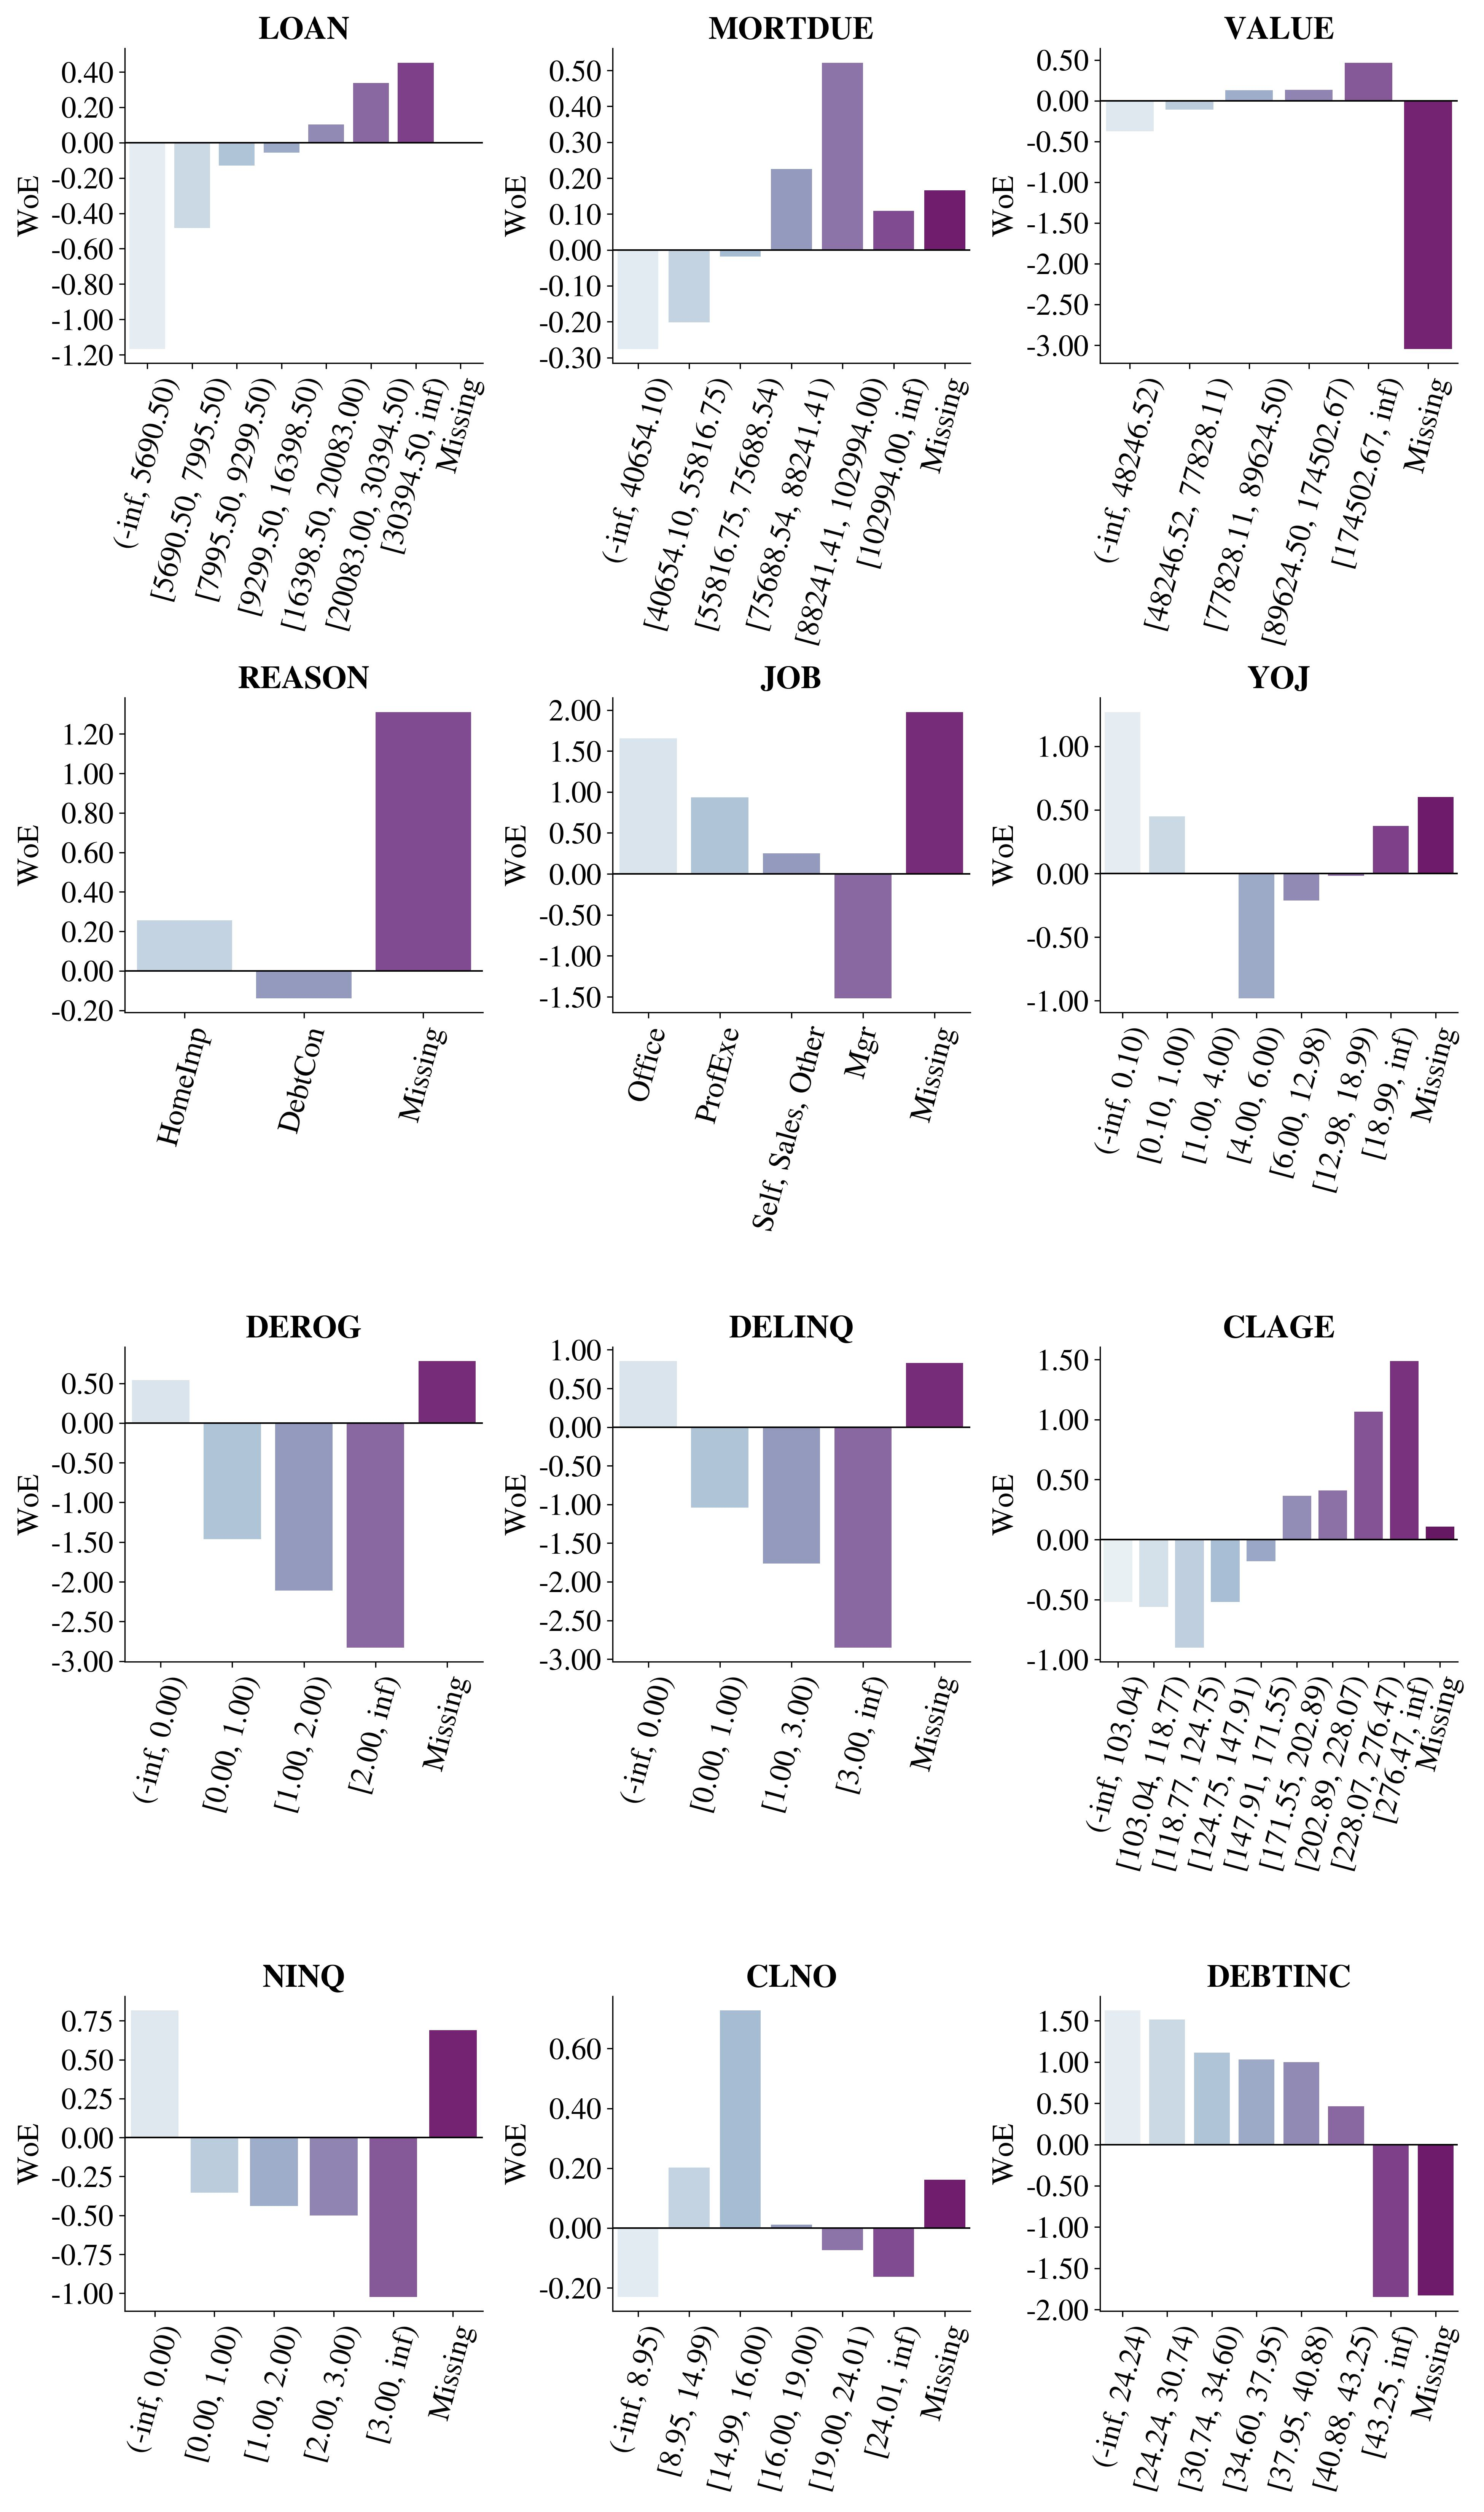
\includegraphics[width=150mm]{Figures/WoE_Distribution.jpg}
    \centering{\begin{source}Author's results in Python.\end{source}}\vspace{-1em}
\end{figure}


\section{Modelling}
Once the data are finally preprocessed, the next step regards the modelling part which includes hyperparameter tuning, feature selection, model selection and model building.

In Python, 8 different machine learning models from \lstinline{Scikit-learn} module are used for the default status prediction, which are:
\begin{itemize}\setlength\itemsep{0em}
    \item Logistic Regression - \lstinline{LogisticRegression from sklearn.linear_model},
    \item Decision Tree - \lstinline{DecisionTreeClassifier from sklearn.tree},
    \item Gaussian Naive Bayes - \lstinline{GaussianNB from sklearn.naive_bayes},
    \item K-Nearest Neighbors - \lstinline{KNeighborsClassifier from sklearn.neighbors},
    \item Random Forest - \lstinline{RandomForestClassifier from sklearn.ensemble},
    \item Gradient Boosting - \lstinline{GradientBoostingClassifier from sklearn.ensemble},
    \item Support Vector Machine - \lstinline{SVC from sklearn.svm},
    \item Neural Network - \lstinline{MLPClassifier from sklearn.neural_network}.
\end{itemize}

\subsection{Hyperparameter Bayesian Optimization}

Instead of using models with default hyperparameters, it is deemed desired to choose optimal hyperparameter values in order to boost model's performance.
One would use Grid Search or Random Search which are commonly used in hyperparameter tuning. Nonetheless, these methods are computationally expensive and do not guarantee to find the global optimum.
Also they do not consider any information from previous iterations but rather checks all the possible hyperparameters combinations or randomly chooses hyperparameters combinations, respectively.

Therefore, Bayesian Optimization is used for hyperparameter tuning instead of Grid Search or Random Search, as a probabilistic model using Gaussian Process is used to approximate the objective function, which we want to target.
Such hyperparameter tuning approach uses Bayesian inference to update prior distribution over hyperparameters' values based on the result of previous iterations and uses resulting posterior distribution to sample guide the selection of the next set of hyperparameters to evaluate.\footnote{Theory behind Bayesian Optimization will be described later}.

In Python, a custom function \lstinline{bayesian_optimization()} is used which further uses \lstinline{BayesSearchCV} class from \lstinline{Scikit-optimize} module with 10-fold stratified cross-validation, 50 iterations while maximizing F1 score. Therefore, each model, the Bayesian Optimization 50 times looks for the best hyperparameters' values while maximizing F1 score where within each iteration, 10-fold stratified cross-validation is used to evaluate the model's F1 score.

The hyperparameter space is defined for each model as follows:
\subsubsection{Logistic Regression}

\begin{table}[H]
    \small
    \setlength{\tabcolsep}{8pt}
    \renewcommand{\arraystretch}{1.3}
    \centering
        \caption[Logistic Regression - Hyperparameter Space]{Logistic Regression - Hyperparameter Space}\label{tab:lrspace}
        \begin{tabular}{ll}
    \toprule
    \textbf{Hyperparameter} & \textbf{Space}\\
    \midrule
    \hline
    Intercept & True, False \\
    $C$ factor & <$1\times10^{-6}$, 5>\\
    Penalty & L1, L2, Elastic Net, None \\
    Solver & lbfgs, liblinear, newton-cg, sag, saga \\
    Class weight & None, balanced \\
    L1 ratio & <0, 1> \\
    Intercept scaling & True, False  \\
    \hline
    \bottomrule
    \end{tabular}
    \vspace{0.7em}

    \centering{\begin{source}Author's results in Python.\end{source}}\vspace{-1em}
\end{table}


\subsubsection{Decision Tree}

\begin{table}[H]
    \small
    \setlength{\tabcolsep}{8pt}
    \renewcommand{\arraystretch}{1.3}
    \centering
        \caption[Decision Tree - Hyperparameter Space]{Decision Tree - Hyperparameter Space}\label{tab:dtspace}
        \begin{tabular}{ll}
    \toprule
    \textbf{Hyperparameter} & \textbf{Space}\\
    \midrule
    \hline
    Criterion & Gini, Entropy \\
    Max depth & <1, 10> \\
    Max features & <1, \verb|len(X.columns)|>  \\
    \hline
    \bottomrule
    \end{tabular}
    \vspace{0.7em}

    \centering{\begin{source}Author's results in Python.\end{source}}\vspace{-1em}
\end{table}

\subsubsection{Gaussian Naive Bayes}

\begin{table}[H]
    \small
    \setlength{\tabcolsep}{8pt}
    \renewcommand{\arraystretch}{1.3}
    \centering
        \caption[Gaussian Naive Bayes - Hyperparameter Space]{Gaussian Naive Bayes  - Hyperparameter Space}\label{tab:gnbspace}
        \begin{tabular}{ll}
    \toprule
    \textbf{Hyperparameter} & \textbf{Space}\\
    \midrule
    \hline
    Variance smoothing & <$1\times 10^{-9}$, $1\times 10^{-6}$> \\
    \hline
    \bottomrule
    \end{tabular}
    \vspace{0.7em}

    \centering{\begin{source}Author's results in Python.\end{source}}\vspace{-1em}
\end{table}



\subsubsection{K-Nearest Neighbors}

\begin{table}[H]
    \small
    \setlength{\tabcolsep}{8pt}
    \renewcommand{\arraystretch}{1.3}
    \centering
        \caption[K--Nearest Neighbors - Hyperparameter Space]{K--Nearest Neighbors - Hyperparameter Space}\label{tab:knnspace}
        \begin{tabular}{ll}
    \toprule
    \textbf{Hyperparameter} & \textbf{Space}\\
    \midrule
    \hline
    \# neighbors & <5, 20> \\
    Weights & Uniform, Distance \\
    Algorithm & Ball Tree, KD Tree, Brute, Auto \\
    Metric & Euclidean, Manhattan, Cityblock, Minkowski \\
    \hline
    \bottomrule
    \end{tabular}
    \vspace{0.7em}

    \centering{\begin{source}Author's results in Python.\end{source}}\vspace{-1em}
\end{table}

\subsubsection{Random Forest}

\begin{table}[H]
    \small
    \setlength{\tabcolsep}{8pt}
    \renewcommand{\arraystretch}{1.3}
    \centering
        \caption[Random Forest - Hyperparameter Space]{Random Forest - Hyperparameter Space}\label{tab:rfspace}
        \begin{tabular}{ll}
    \toprule
    \textbf{Hyperparameter} & \textbf{Space}\\
    \midrule
    \hline
    \# estimators & <100, 1000> \\
    Criterion & Gini, Entropy, Log Loss \\
    Max depth & <1, 10> \\
    Max features & <1, \verb|len(X.columns)|>  \\
    Class weight & None, balanced, subsample balanced \\
    Bootstrap & True, False \\
    CCP alpha & <$1 \times 10^{-12}$, 0.5> \\
    \hline
    \bottomrule
    \end{tabular}
    \vspace{0.7em}

    \centering{\begin{source}Author's results in Python.\end{source}}\vspace{-1em}
\end{table}

\subsubsection{Gradient Boosting}

\begin{table}[H]
    \small
    \setlength{\tabcolsep}{8pt}
    \renewcommand{\arraystretch}{1.3}
    \centering
        \caption[Gradient Boosting - Hyperparameter Space]{Gradient Boosting - Hyperparameter Space}\label{tab:gbspace}
        \begin{tabular}{ll}
    \toprule
    \textbf{Hyperparameter} & \textbf{Space}\\
    \midrule
    \hline
    \# estimators & <100, 1000> \\
    Criterion & Friedman MSE, Squared Error \\
    Max depth & <1, 10> \\
    Max features & <1, \verb|len(X.columns)|>  \\
    Loss & Log Loss, Exponential \\
    Learning rate & <0.0001, 0.2> \\
    \hline
    \bottomrule
    \end{tabular}
    \vspace{0.7em}

    \centering{\begin{source}Author's results in Python.\end{source}}\vspace{-1em}
\end{table}

\subsubsection{Support Vector Machine}


\begin{table}[H]
    \small
    \setlength{\tabcolsep}{8pt}
    \renewcommand{\arraystretch}{1.3}
    \centering
        \caption[Support Vector Machine - Hyperparameter Space]{Support Vector Machine - Hyperparameter Space}\label{tab:svmspace}
        \begin{tabular}{ll}
    \toprule
    \textbf{Hyperparameter} & \textbf{Space}\\
    \midrule
    \hline
    C factor & <$1\times 10^{-6}$, 5> \\
    Kernel & Linear, Poly, RBF, Sigmoid \\
    Degree & <1, 10> \\
    Gamma & scale, auto \\
    Shrinking & True, False \\
    Decision function shape & OVR, OVO \\
    tol & <$1\times 10^{-9}$, $1\times 10^{-3}$> \\
    Class weight & balanced, None \\
    \hline
    \bottomrule
    \end{tabular}
    \vspace{0.7em}

    \centering{\begin{source}Author's results in Python.\end{source}}\vspace{-1em}
\end{table}


\subsubsection{Neural Network}

\begin{table}[H]
    \small
    \setlength{\tabcolsep}{8pt}
    \renewcommand{\arraystretch}{1.3}
    \centering
        \caption[Multi Layer Percepton - Hyperparameter Space]{Multi Layer Percepton - Hyperparameter Space}\label{tab:mlpspace}
        \begin{tabular}{ll}
    \toprule
    \textbf{Hyperparameter} & \textbf{Space}\\
    \midrule
    \hline
    Hidden layer size & <5, 500> \\
    Activation function & Identity, Logistic, Tanh, ReLU \\
    Solver & Adam, SGD, LBFGS \\
    Learning rate & Constant, Adaptive, Invscaling \\
    \hline
    \bottomrule
    \end{tabular}
    \vspace{0.7em}

    \centering{\begin{source}Author's results in Python.\end{source}}\vspace{-1em}
\end{table}


\subsection{Feature Selection}
\label{subsec:feature-selection}

In subsection, the process of selecting optimal features is described. Instead of using all the features in dataset, only the most relevant are chosen and the noisy ones are eliminated.

For such case, the Forward Sequential Feature Selection is used. The approach is following - for each model:

\begin{enumerate}\setlength\itemsep{0em}
    \item tune the model with Bayesian Optimization;
    \item use such tuned model as an input estimator within Forward Sequential Feature Selection;
    \item get the best features for each model.
\end{enumerate}

Thus, when having $n$ input models, it returns $n$  subsets of optimal features, one per each model.

In Python, a custom function \lstinline{SFS_feature_selection()} is used which further uses another custom function defined previously \lstinline{bayesian_optimization()} for tuning the model, and \lstinline{SequentialFeatureSelector} class from \lstinline{Scikit-learn} for feature selection.
\lstinline{SequentialFeatureSelector} class is predetermined with the \texttt{forward} direction, 10--fold stratified cross validation while maximizing F1 score.

Instead of choosing a fixed number of features, \lstinline{SequentialFeatureSelector} class also allows to choose a variable number of features due to the early stopping (\texttt{tol} paramater) - The \lstinline{SequentialFeatureSelector} stops adding new features into optimal subset if the objective score is not incremented by at least \texttt{tol} between two consecutive feature additions\citep{scikit-learn-sequential-feature-selector}.
The \texttt{tol} parameter is set to the number close to zero indicating that the feature selection should stop adding new features if the F1 score is not increasing between two consecutive feature additions.

The custom function \lstinline{SFS_feature_selection()} iterively prints the process of the feature selection for in order to keep the track of such process as it is depicted in \autoref{fig:fsprint}.
Particularly, it prints which step model and which step is currently being executed (whether it is Bayesian Optimization or Feature Selection), the execution time and the selected features for each model.

\begin{figure}[H]
    \centering
    \caption{Feature Selection Print Statement}\vspace{0.5em}
    \label{fig:fsprint}\
    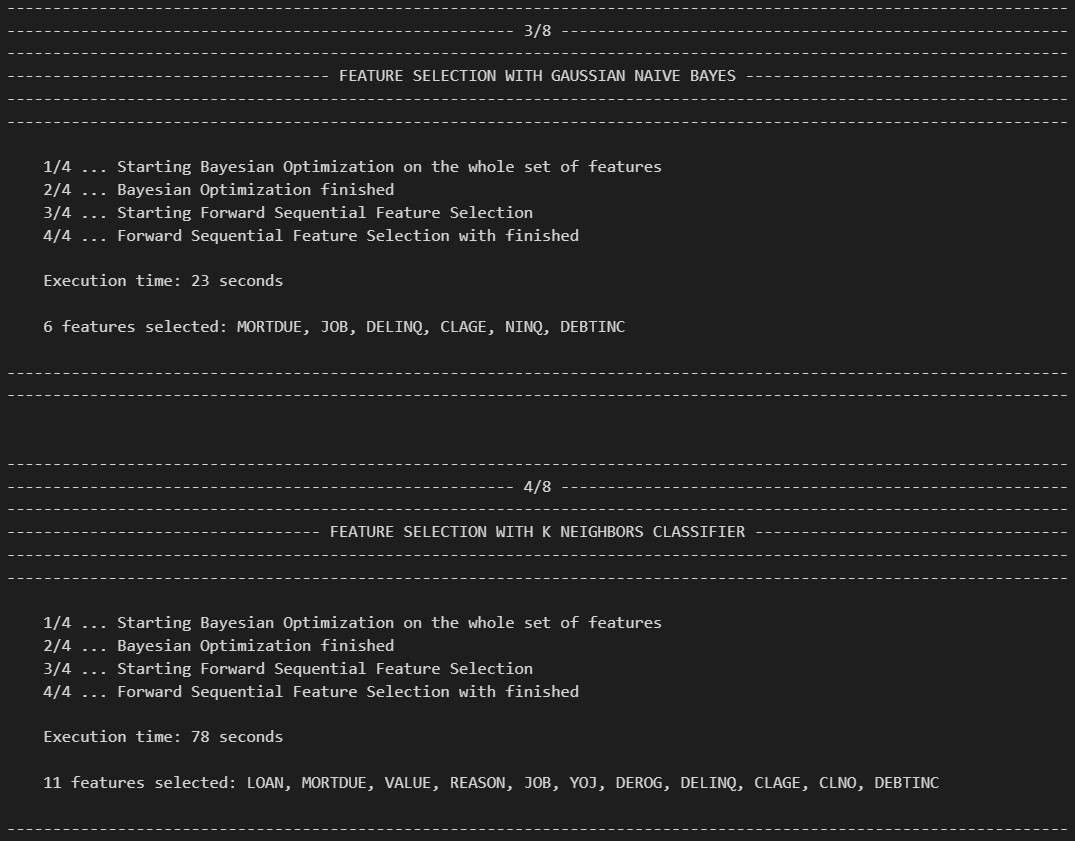
\includegraphics[width=140mm]{Figures/fs_print.jpg}
    \centering{\begin{source}Author's results in Python.\end{source}}\vspace{-1em}
\end{figure}


The following \autoref{fig:fsrec} depicts the reccurrence of the selected features. As can be seen, features such as \texttt{CLAGE}, \texttt{DEBTINC}, \texttt{JOB} and \texttt{REASON} were selected by each model. 
On the other hand, features such as \texttt{LOAN} and \texttt{REASON} were selected by only 4 times. Therefore, we can expect that such features which were selected every time will have high importance in predictions. \textit{the figure will be adjusted, it has been incorrectly exported}.

\begin{figure}[H]
    \centering
    \caption{Reccurrence of Selected Features}\vspace{0.5em}
    \label{fig:fsrec}\
    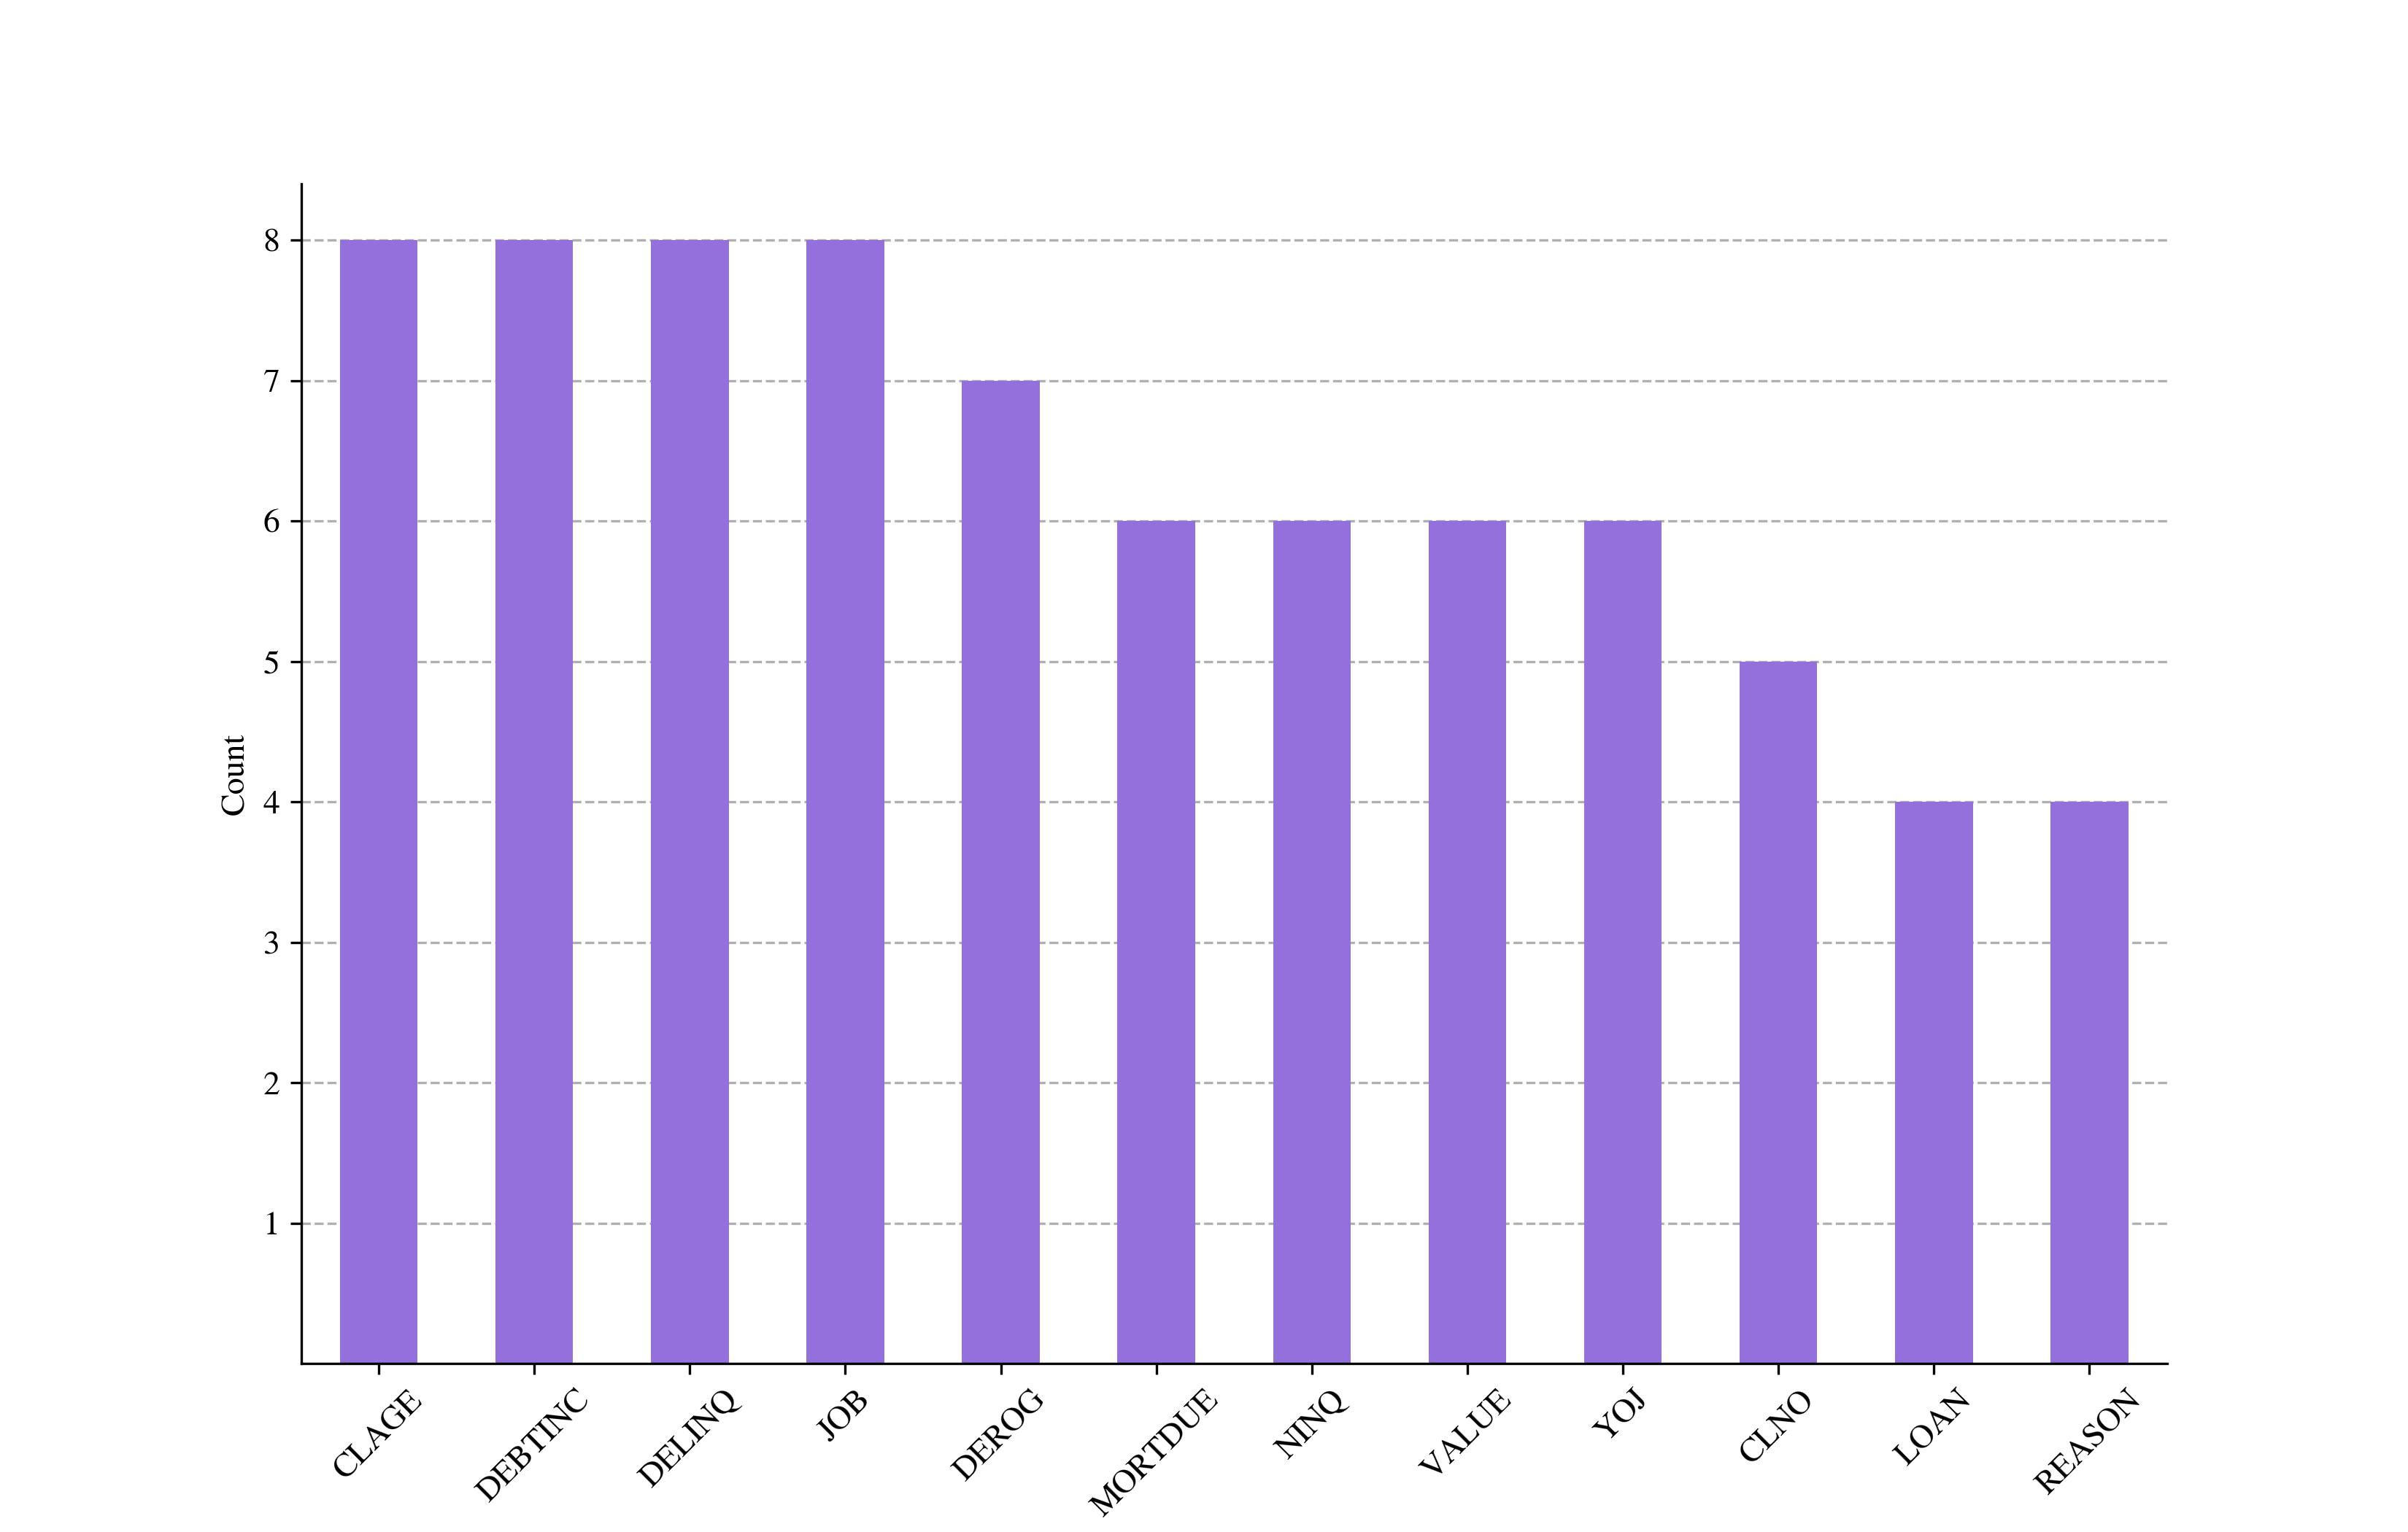
\includegraphics[width=150mm]{Figures/Recurrence_Selected_Features.jpg}
    \centering{\begin{source}Author's results in Python.\end{source}}\vspace{-1em}
\end{figure}


According to \autoref{fig:fsdistmod}, models such as K--Nearest Neighbors, Random Forest, Gradient Boosting and Support Vector Machine chose all the features from the dataset. On the other hand, Gaussian Naive Bayes chose only 6. It seems to be that most of the features are important as each model has selected a higher amount of features. \textit{the figure will be adjusted, it has been incorrectly exported}.

\begin{figure}[H]
    \centering
    \caption{Distribution of Selected Features per Model}\vspace{0.5em}
    \label{fig:fsdistmod}\
    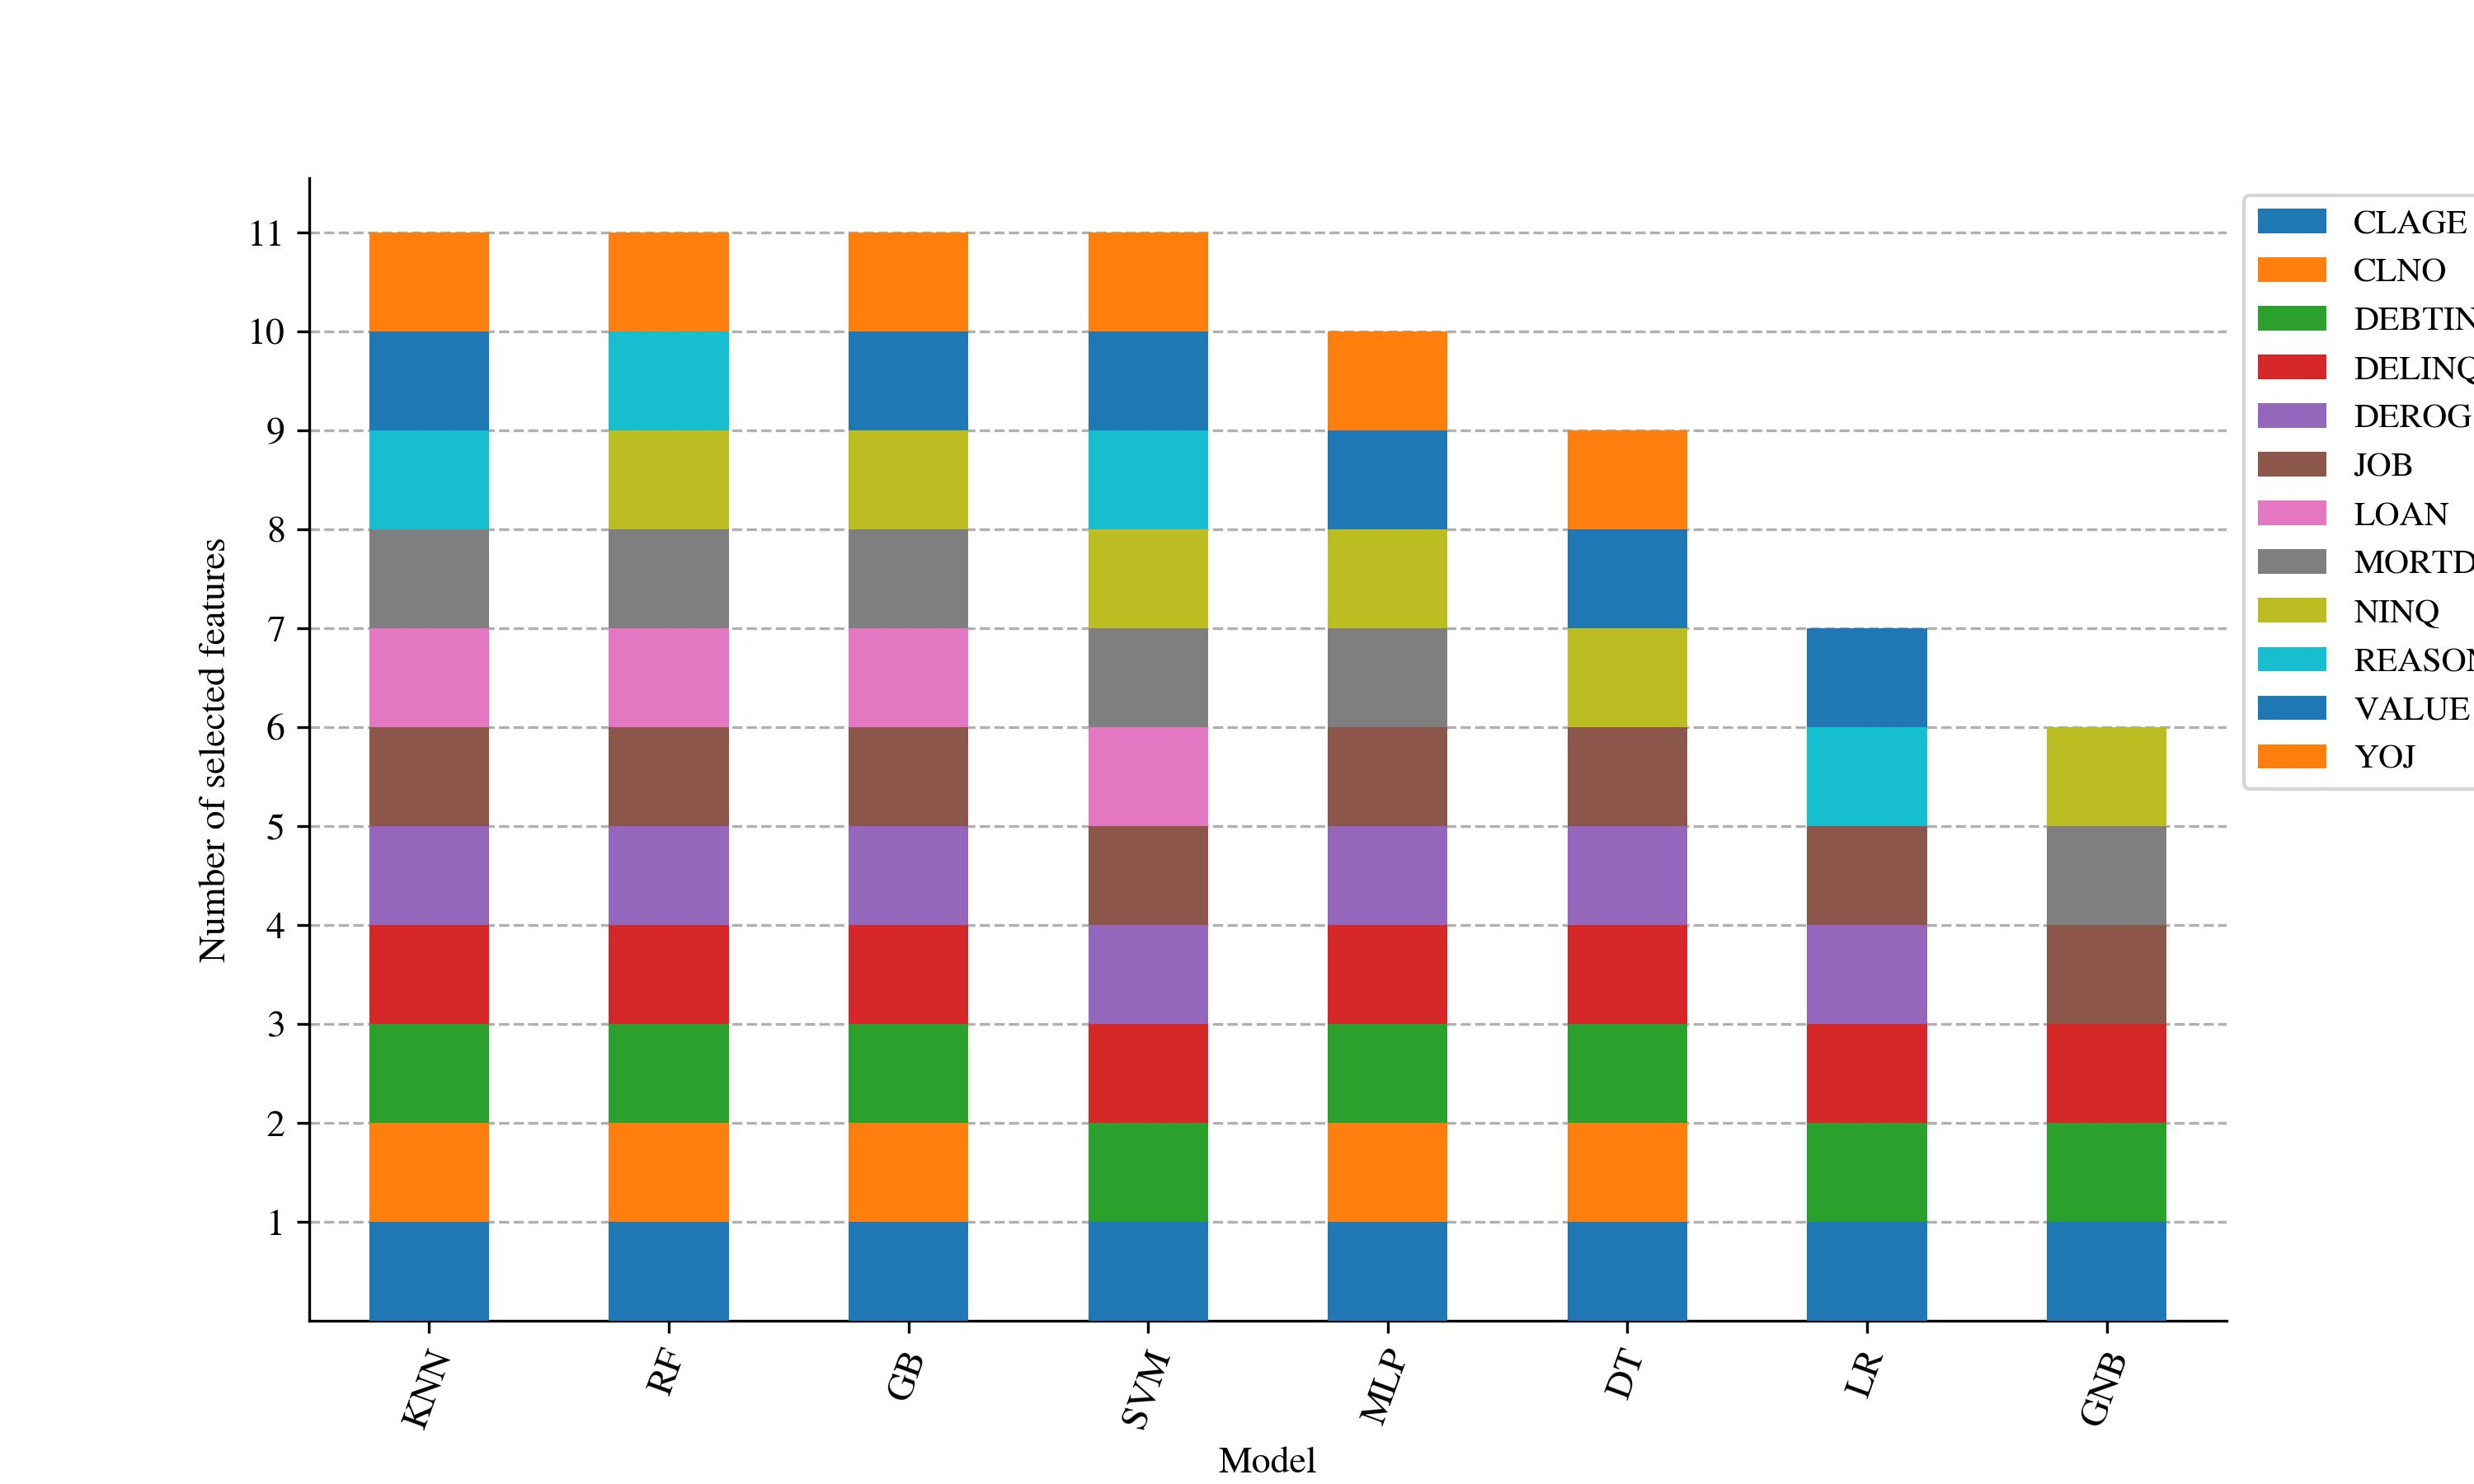
\includegraphics[width=140mm]{Figures/Selected_Features_Distribution.jpg}
    \centering{\begin{source}Author's results in Python.\end{source}}\vspace{-1em}
\end{figure}

\subsection{Model Selection}

In combination with the pre--selected subsets of features, the next step regards the selection of the final model. The process is following:

\begin{enumerate}\setlength\itemsep{0em}
    \item tune each model on each subset of optimal features (selected within Feature Selection) with Bayesian Optimization on the training set.
    \item evaluate tuned model on the validation set.
\end{enumerate}

Thus, when having $n$ input models and $m$ subsets of selected features, we get $n \times m$ tuned models.
$m \leq n$ because we exclude duplicated subset of selected features which can occur when more than one model choose the same subset(s) of features.
Since there are 8 input models and 8 unique subsets of selected features, the total number of tuned models is 64.

Further, for each model, we evalute it on the validation set by computing following metrics scores and loss functions:
\begin{itemize}\setlength\itemsep{0em}
    \item F1 score,
    \item Precision,
    \item Recall,
    \item Accuracy,
    \item AUC,
    \item Somers' D,
    \item Kolmogorov Smirnov Distance,
    \item Matthews Correlation Coefficient,
    \item Jaccard Score,
    \item Brier Score Loss,
    \item Zero-One Loss.
\end{itemize}

Pertaining to the class--based metrics which require predicted classes (and not predicted probability scores), such as F1 score, Precision, Recall, Accuracy, Matthews Correlation Coefficient, Jaccard Score and Zero-One Loss, by default they use a default classifiation threshold of 0.5.
Meaning if the probability score is higher than 0.5, it will be encoded as class 1 and otherwise. 
Note that 0.5 clasification threshold does not have to be valid for real life use cases. Therefore, it is deemed desired to calculate an optimal threshold instead of using the default one.
One way how to achieve this is to use Younden index which is derived from ROC curve 

\begin{equation}\label{eq}
J = \text{TPR} - \text{FPR}
\end{equation}


\begin{equation}\label{eq}
    T_{opt} = \text{argmax}_{t \in [0, 1]}(J)
\end{equation}

\begin{figure}[H]
    \centering
    \caption{F1 score distribution}\vspace{0.5em}
    \label{fig:f1dist}\
    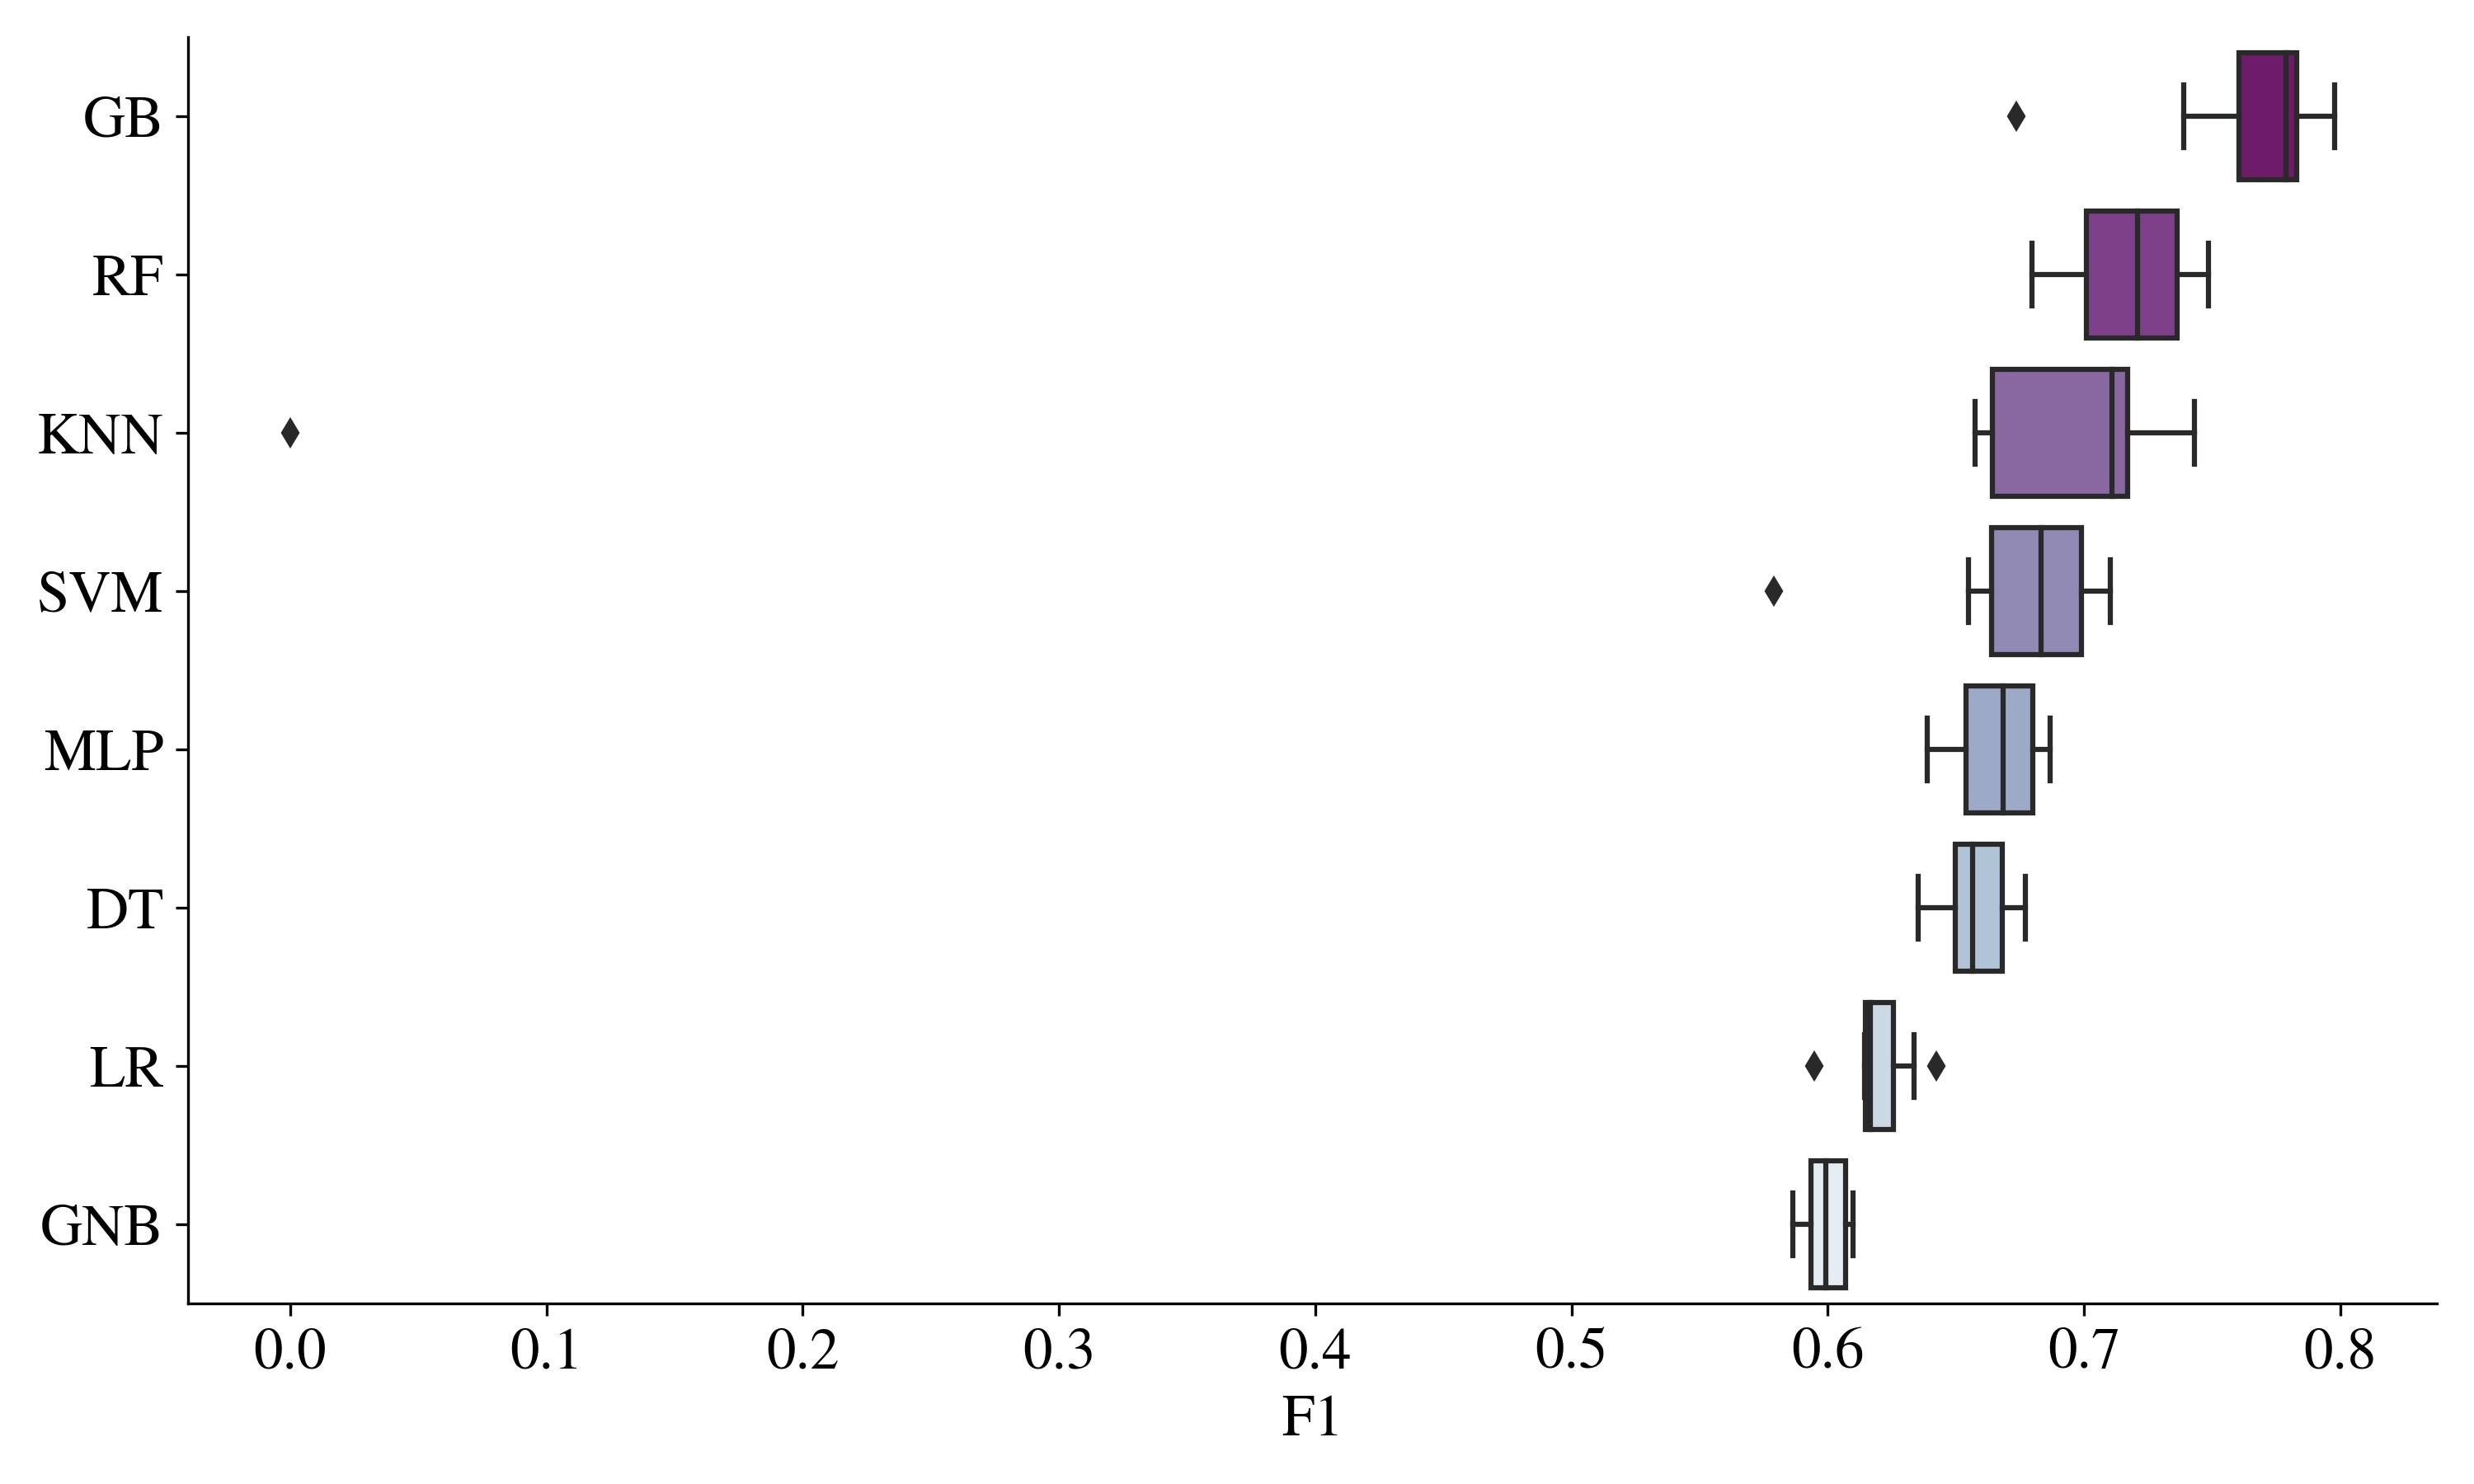
\includegraphics[width=140mm]{Figures/F1_Distribution.jpg}
    \centering{\begin{source}Author's results in Python.\end{source}}\vspace{-1em}
\end{figure}

\begin{figure}[H]
    \centering
    \caption{F1 score distribution - without outliers}\vspace{0.5em}
    \label{fig:f1distclean}\
    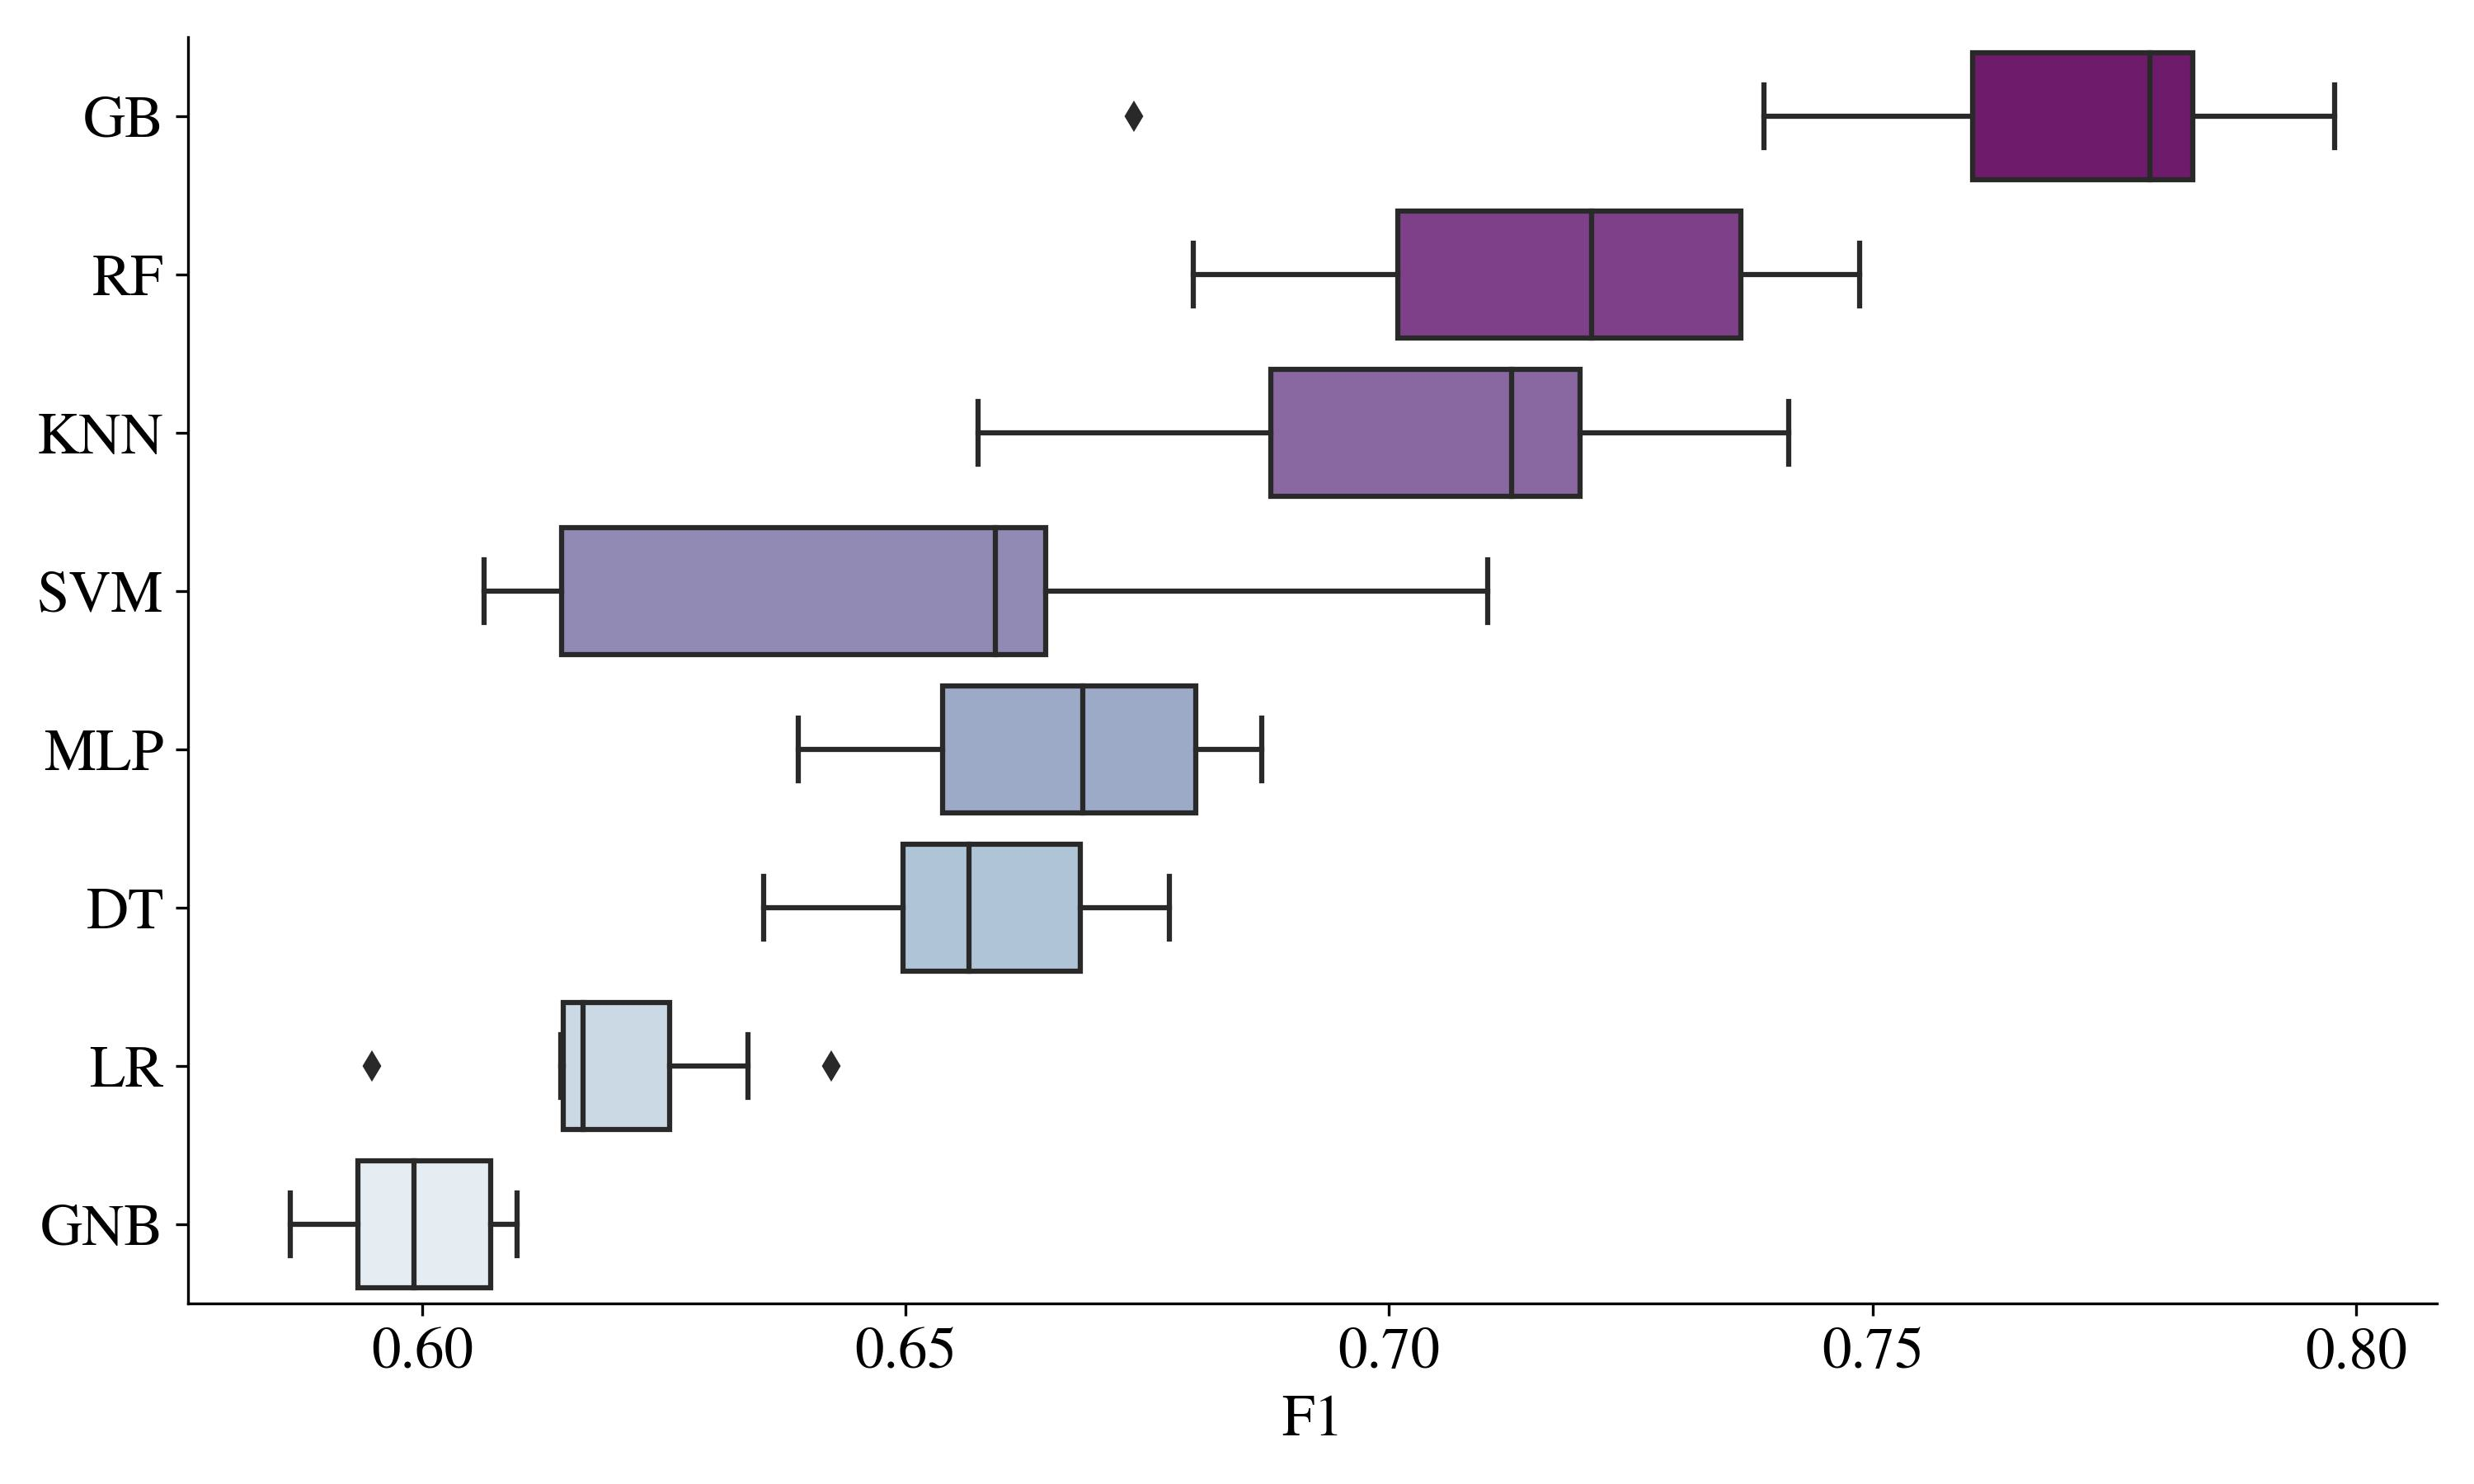
\includegraphics[width=140mm]{Figures/F1_wo_outliers_Distribution.jpg}
    \centering{\begin{source}Author's results in Python.\end{source}}\vspace{-1em}
\end{figure}

\begin{figure}[H]
    \centering
    \caption{Classification Threshold distribution}\vspace{0.5em}
    \label{fig:thresdist}\
    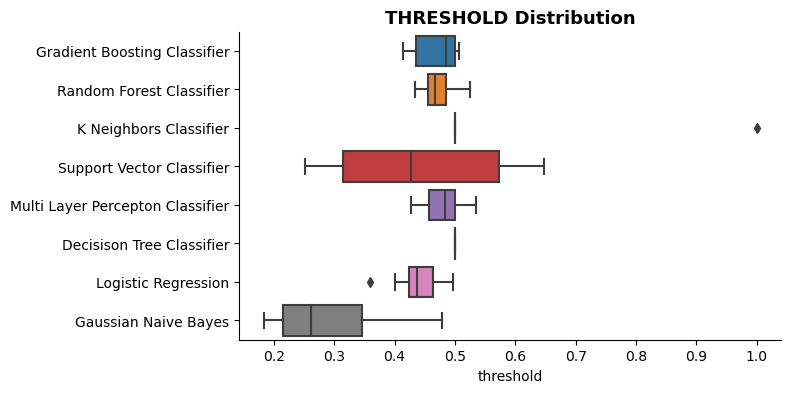
\includegraphics[width=140mm]{Figures/Threshold_Distribution.jpg}
    \centering{\begin{source}Author's results in Python.\end{source}}\vspace{-1em}
\end{figure}


\begin{figure}[H]
    \centering
    \caption{Classification Threshold distribution - without outliers}\vspace{0.5em}
    \label{fig:thresdistclean}\
    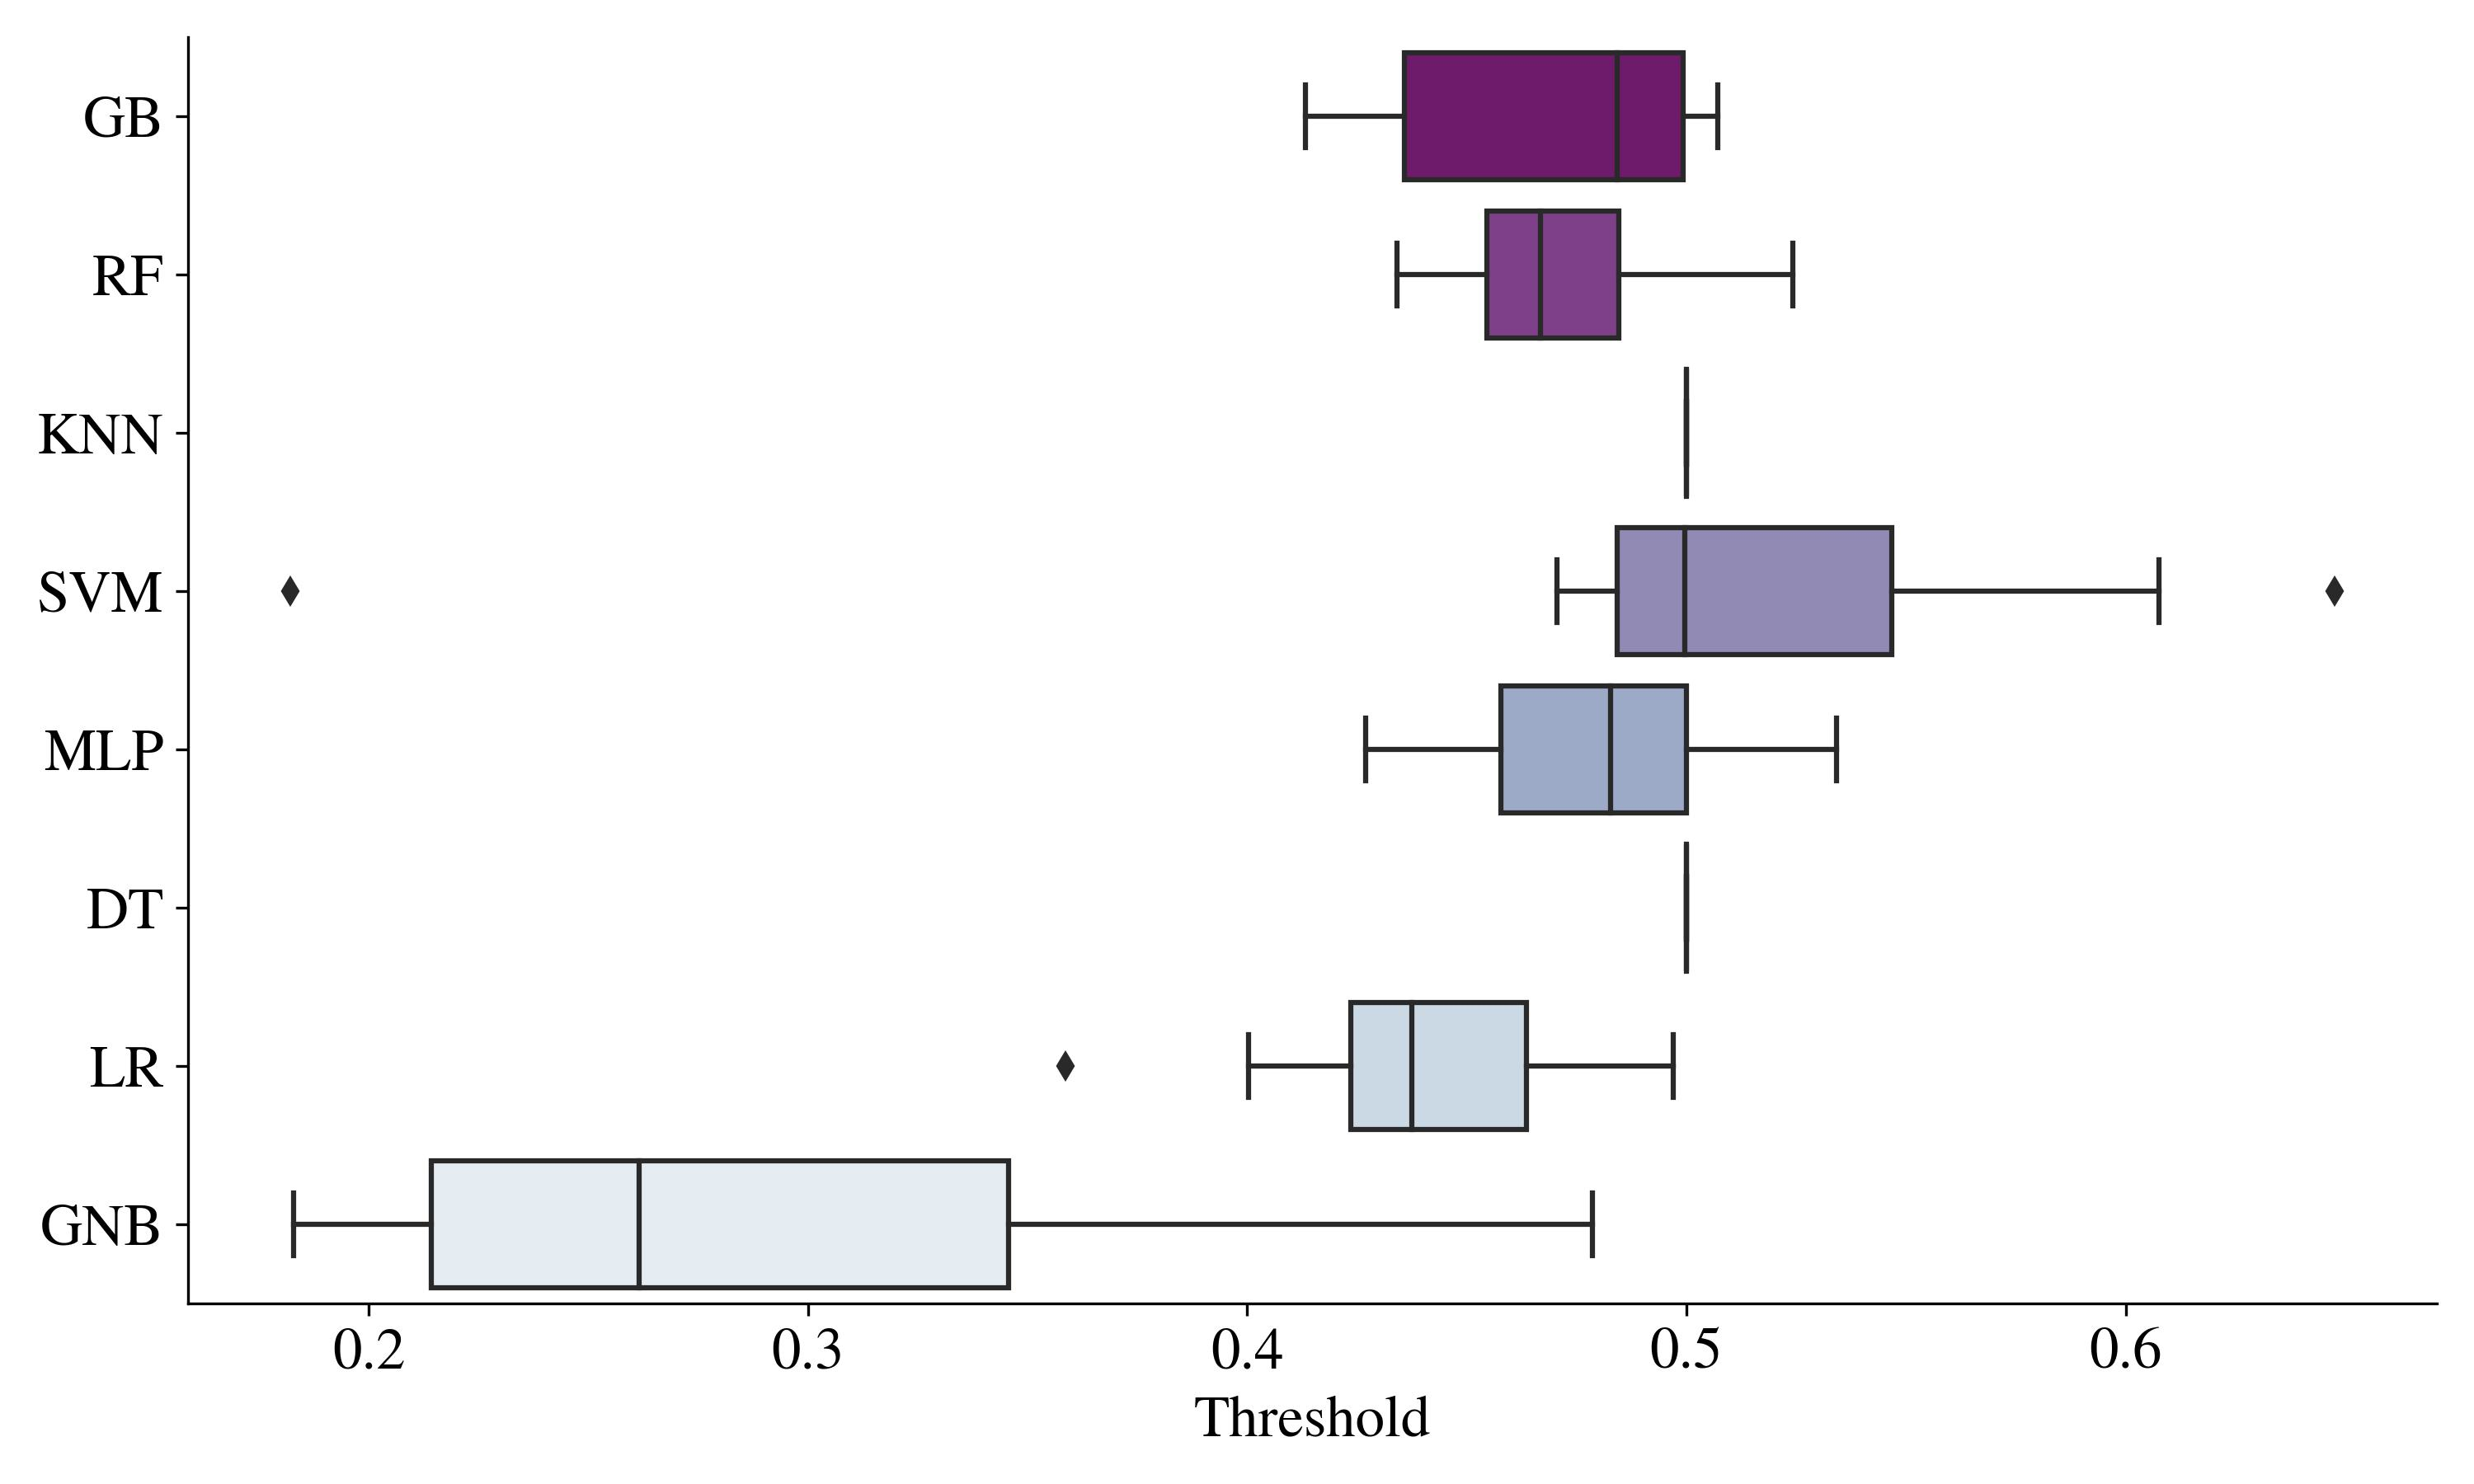
\includegraphics[width=140mm]{Figures/Threshold_wo_outliers_Distribution.jpg}
    \centering{\begin{source}Author's results in Python.\end{source}}\vspace{-1em}
\end{figure}


\begin{figure}[H]
    \centering
    \caption{Execution time distribution}\vspace{0.5em}
    \label{fig:timedist}\
    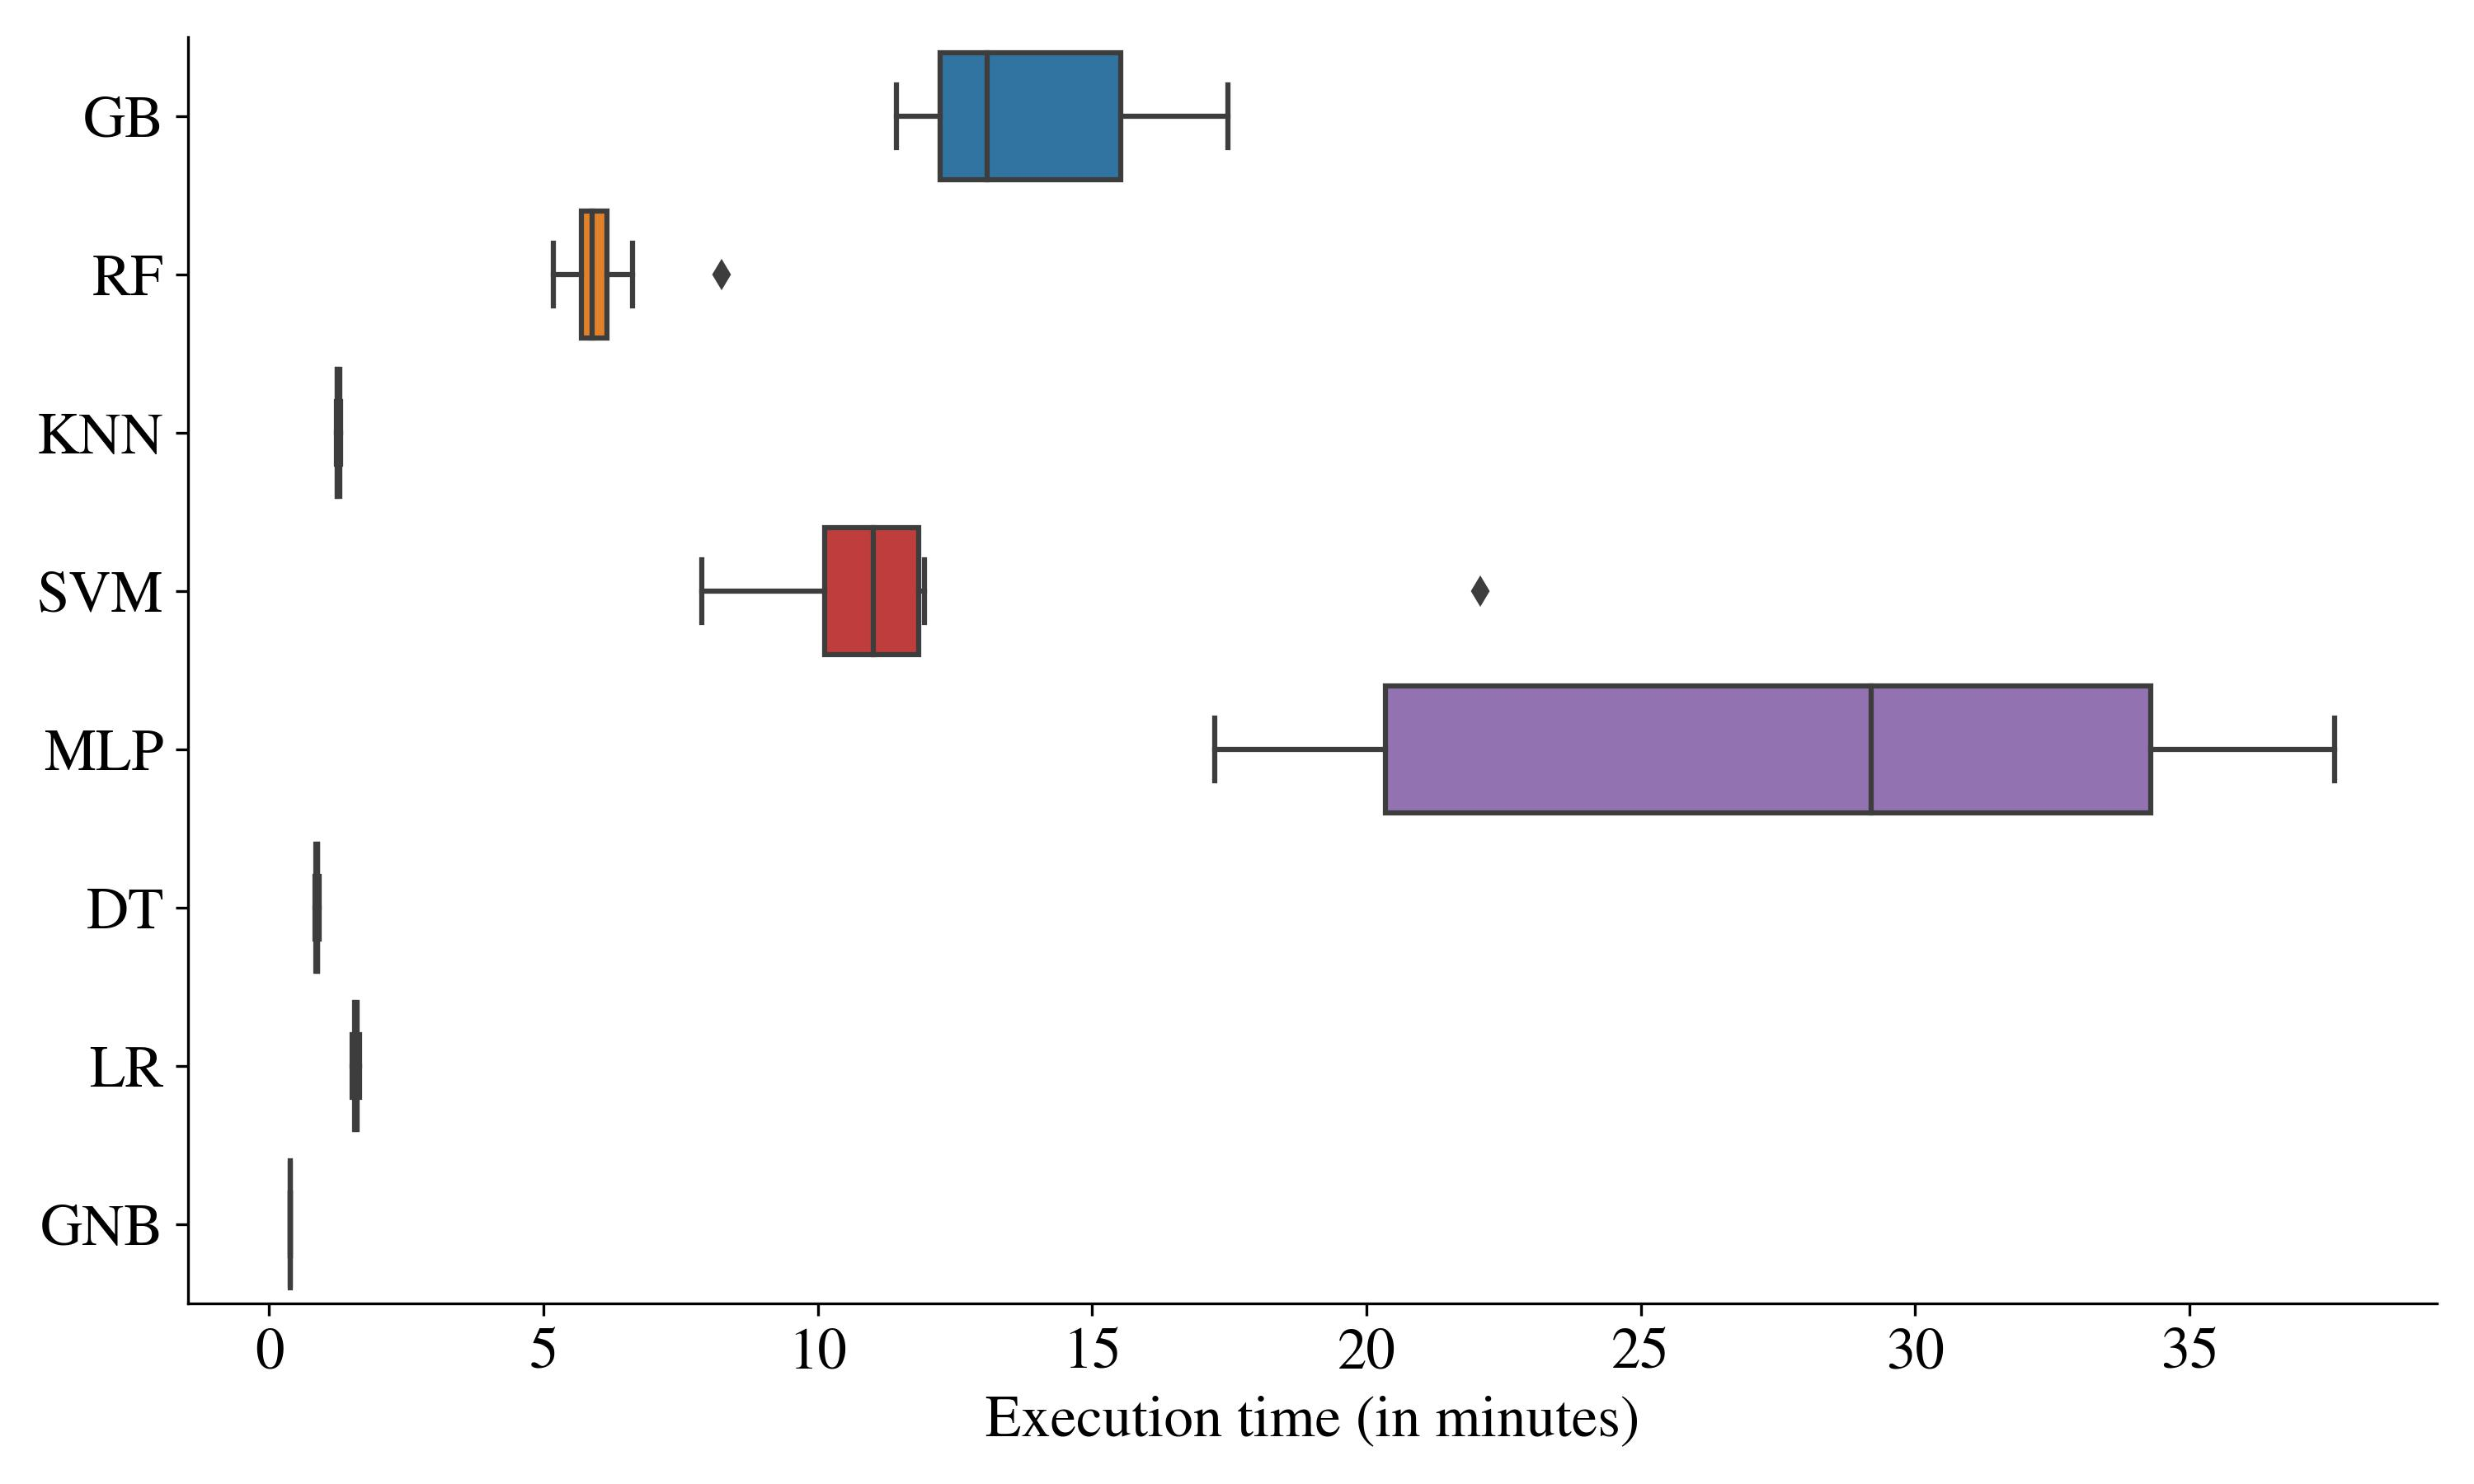
\includegraphics[width=140mm]{Figures/EXECUTION_TIME_Distribution.jpg}
    \centering{\begin{source}Author's results in Python.\end{source}}\vspace{-1em}
\end{figure}


\subsection{Model Building}
\section{Model Evaluation}
\subsection{Confusion Matrix}

\begin{figure}[H]
    \centering
    \caption{Confusion Matrix}\vspace{0.5em}
    \label{fig:confmat}\
    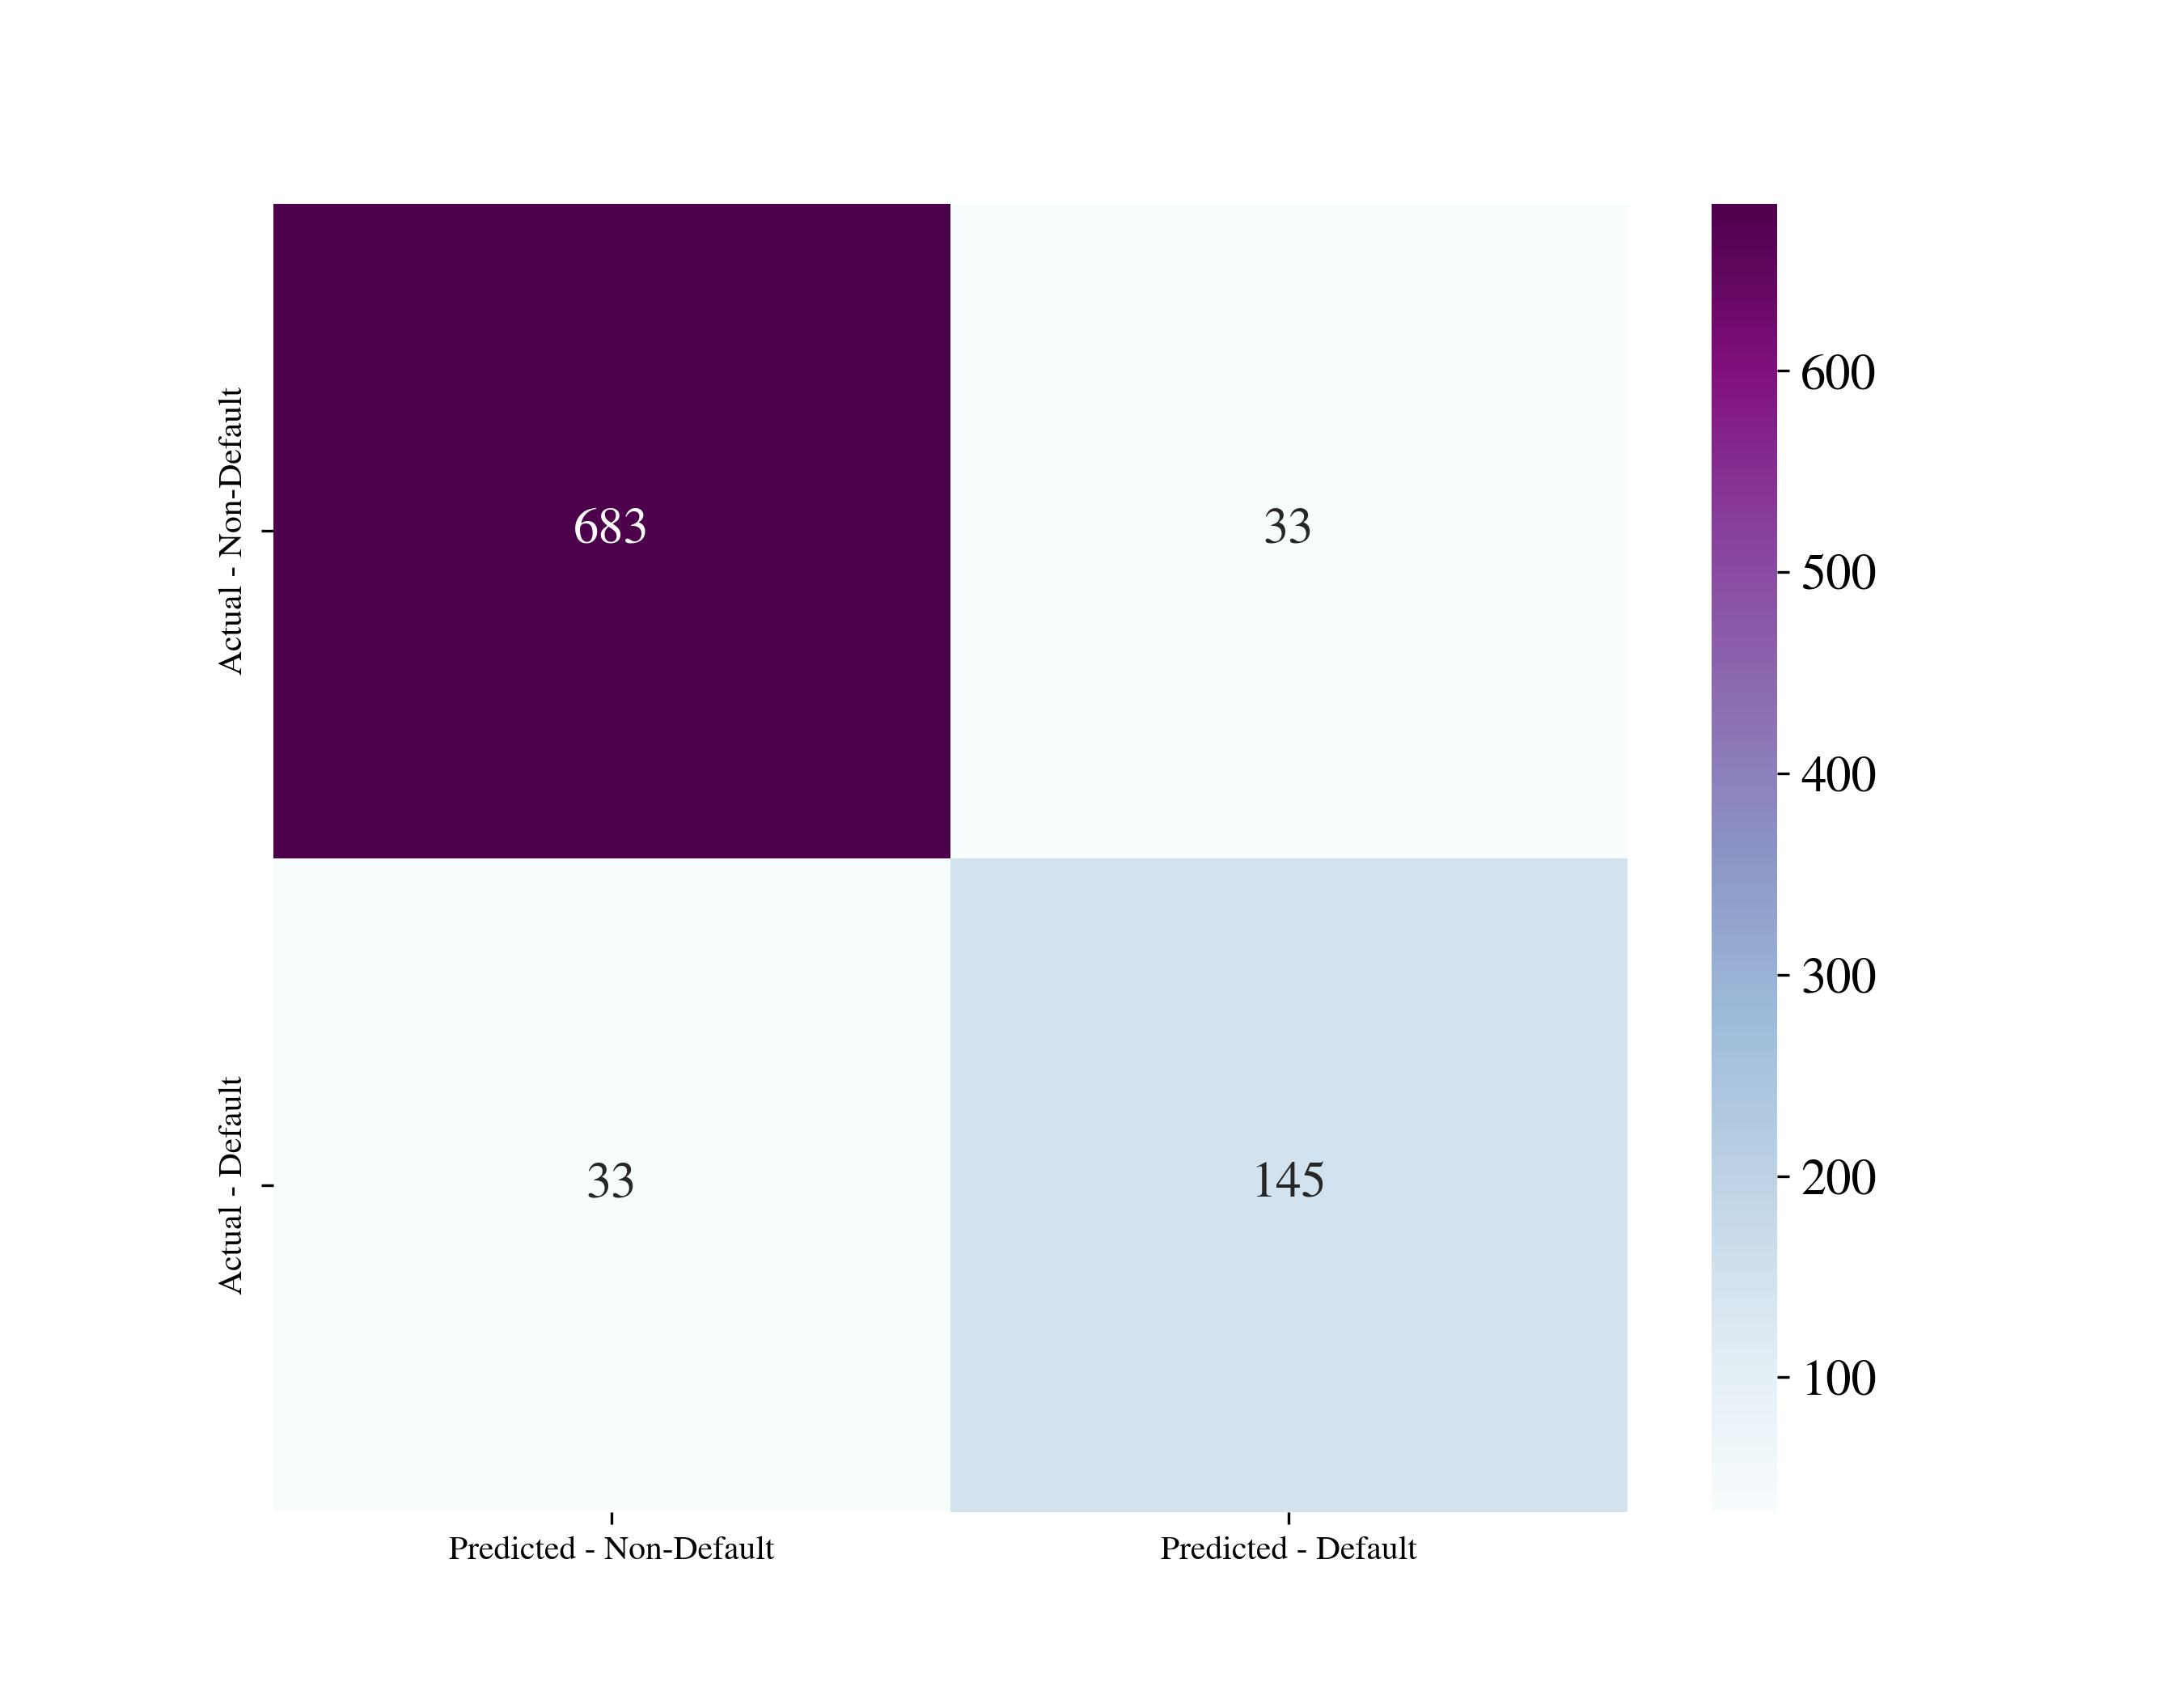
\includegraphics[width=140mm]{Figures/Confusion_Matrix.jpg}
    \centering{\begin{source}Author's results in Python.\end{source}}\vspace{-1em}
\end{figure}

\subsection{Metrics Scores}


    \begin{table}[H]
        \small
        \setlength{\tabcolsep}{8pt}
        \renewcommand{\arraystretch}{1.3}
        \centering
            \caption[Metrics Evaluation]{Metrics Evaluation}\label{tab:metrics eval}
            \begin{tabular}{@{} l r @{\hspace{1cm}} l @{}}
        \toprule
        \textbf{Metric} & \textbf{Value}\\
        \midrule
        \hline
        F1 & 0.8046 \\
        Precision & 0.8235 \\
        Recall & 0.7865 \\
        Accuracy & 0.9239 \\
        AUC & 0.9555 \\
        Somers D & 0.9111 \\
        KS & 0.7885 \\
        MCC & 0.7577 \\
        Jaccard Score & 0.6731 \\
        Brier Score Loss & 0.0617 \\
        Zero-One Loss & 0.0761 \\
        \hline
        \bottomrule
        \end{tabular}
        \vspace{0.35em}

            \centering{\begin{source}Author's results in Python.\end{source}}\vspace{-1em}
\end{table}


\subsection{ROC Curve}

\begin{figure}[H]
    \centering
    \caption{ROC Curve}\vspace{0.5em}
    \label{fig:roc}\
    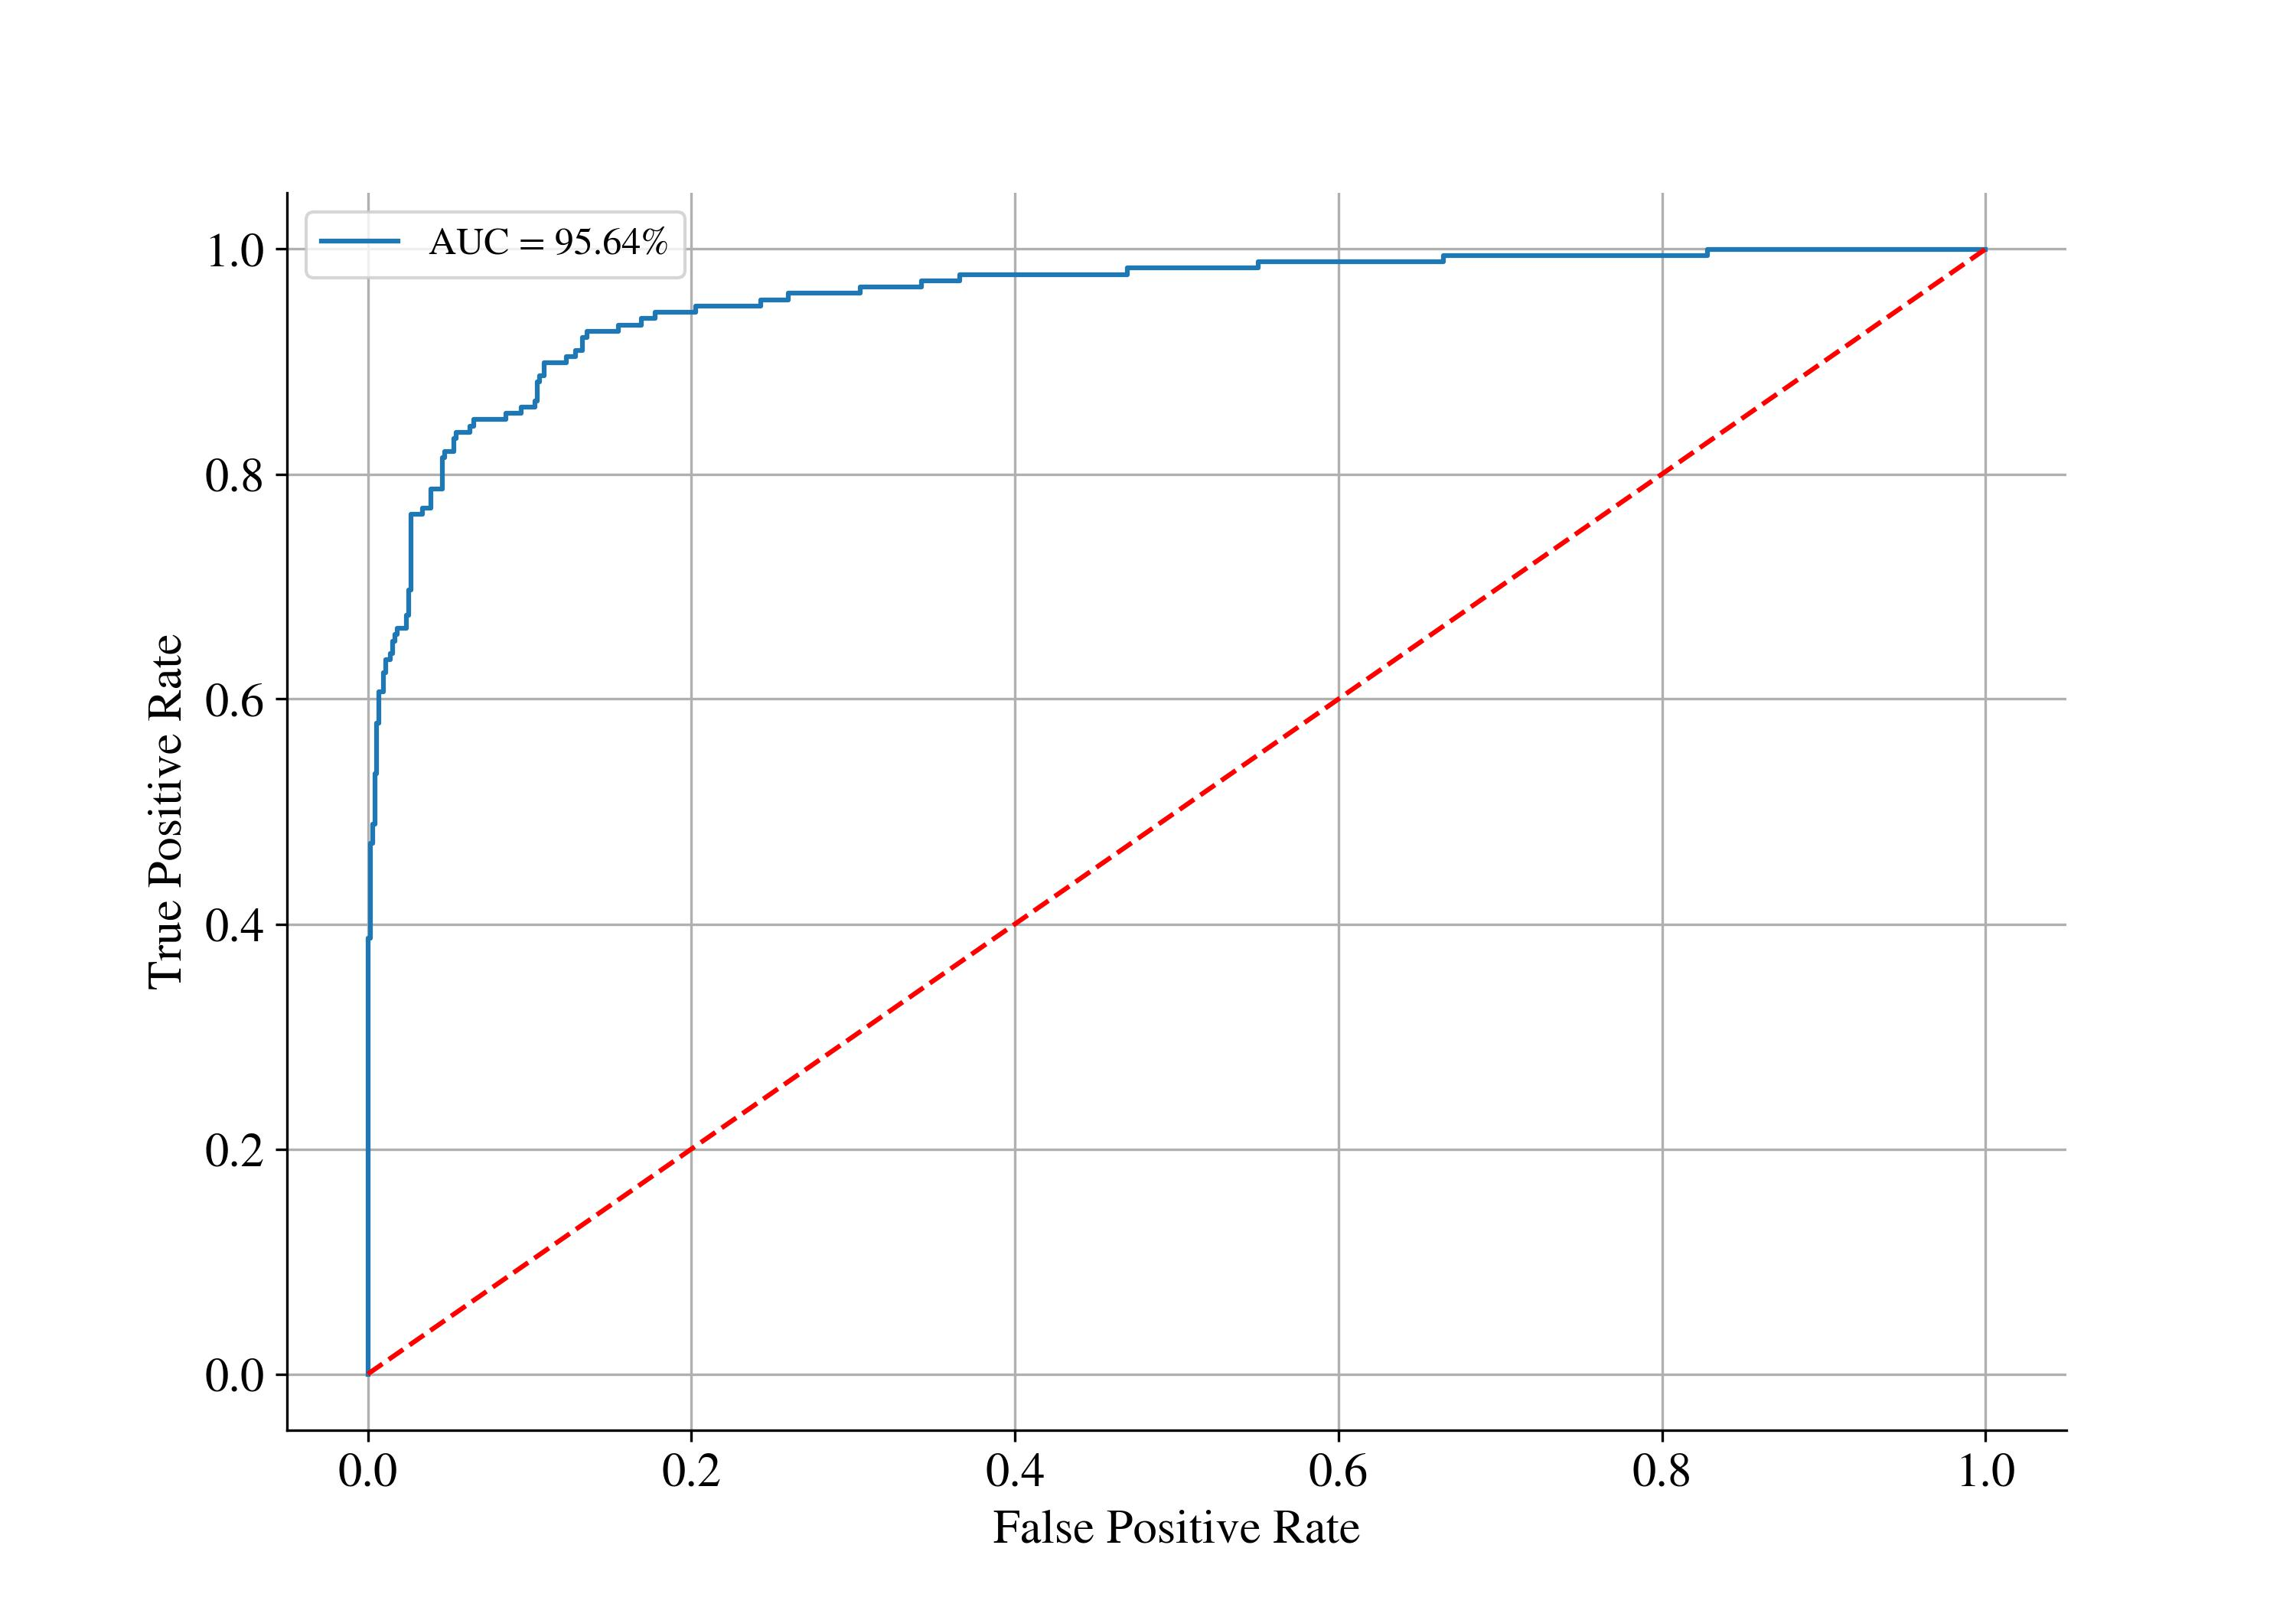
\includegraphics[width=150mm]{Figures/ROC_curve_FINAL.jpg}
    \centering{\begin{source}Author's results in Python.\end{source}}\vspace{-1em}
\end{figure}

\subsection{SHAP Values}

\begin{figure}[H]
    \centering
    \caption{SHAP Summary Plot}\vspace{0.5em}
    \label{fig:shap}\
    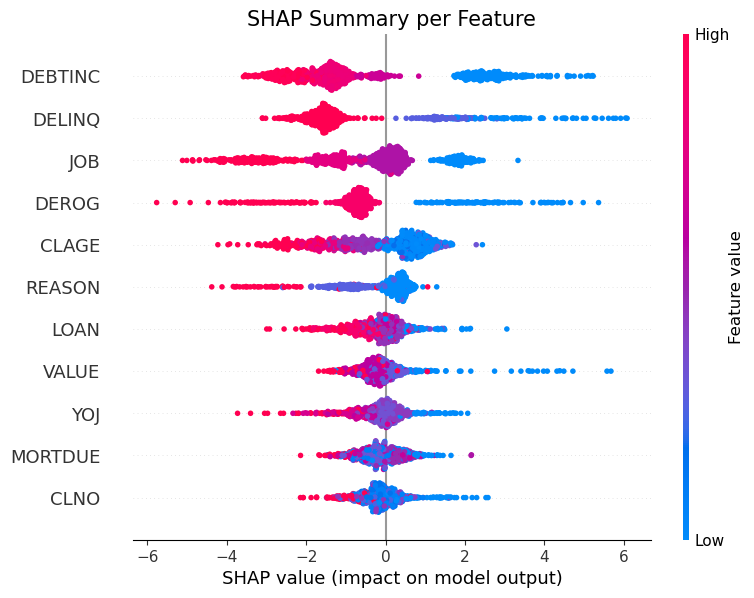
\includegraphics[width=140mm]{Figures/SHAP_values.jpg}
    \centering{\begin{source}Author's results in Python.\end{source}}\vspace{-1em}
\end{figure}

\section{Machine Learning Deployment}
\subsection{Final Model Building}
\subsection{Flask and HTML Web Application}
Once the final model is trained or built, it can be deployed into a production and monitored.

For machine learning deployment in this case, the model is deployed into a web application using Flask and HTML. 

\begin{figure}[H]
    \centering
    \caption{Flask Web Application Form}\vspace{0.5em}
    \label{fig:shap}\
    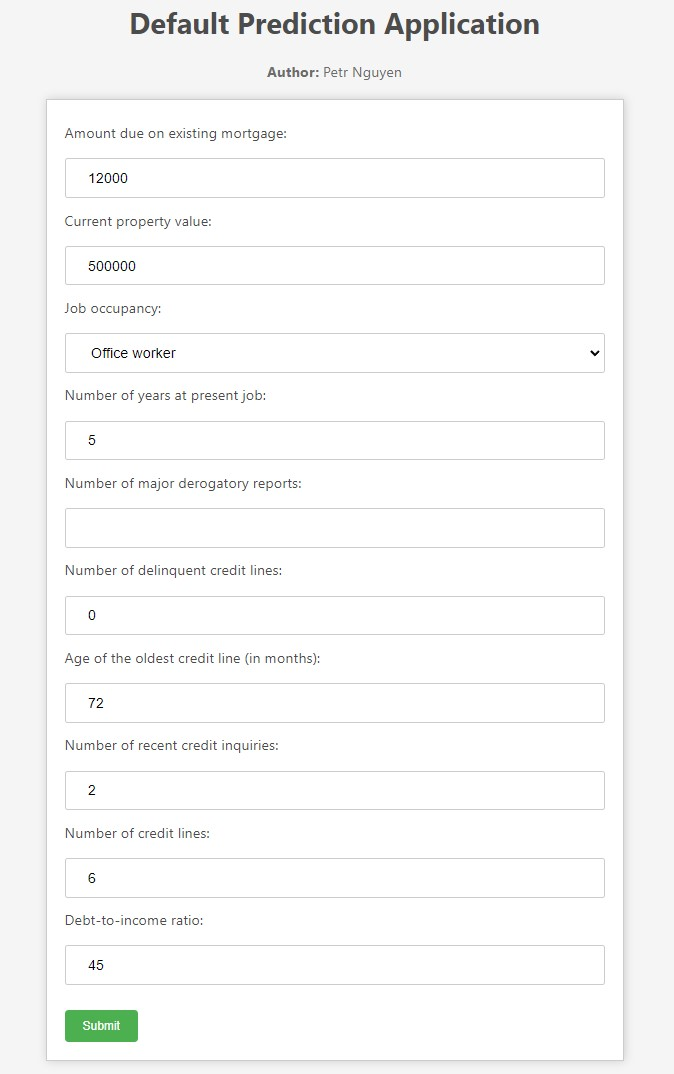
\includegraphics[width=100mm]{Figures/flask_app_form.jpg}

    \centering{\begin{source}Author's results in Python.\end{source}}\vspace{-1em}
\end{figure}


\begin{figure}[H]
    \centering
    \caption{Flask Web Application - Prediction Result}\vspace{0.5em}
    \label{fig:shap}\
    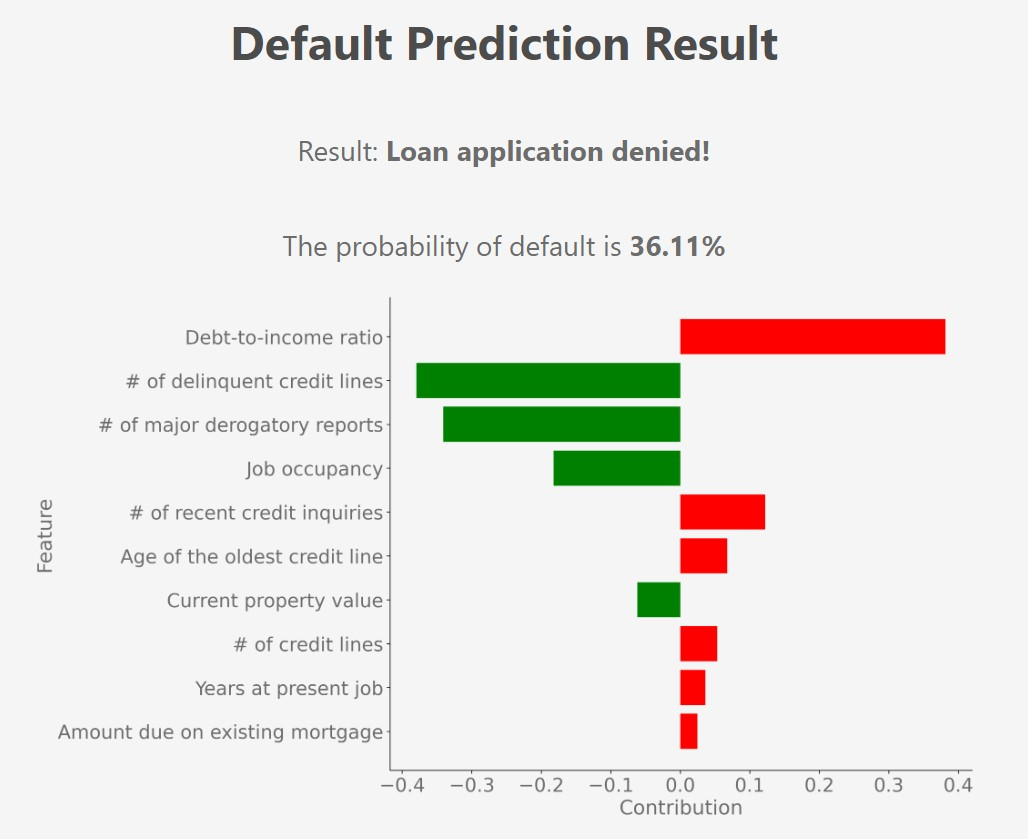
\includegraphics[width=90mm]{Figures/flask_app_result.jpg}

    \centering{\begin{source}Author's results in Python.\end{source}}\vspace{-1em}
\end{figure}

Itemization and Environments

Many people use simple n-dash in many occasions -- like this --, where however typographic convention---it looks a bit strange at first sight---requires m-dash.
Text text text text text text \citet{Haufler2006}. 

Text text text text text text \citet{Wells2001}. Let us describe the following animals:

\begin{description}
\item[Item 1] Text.
\item[Item 2] Text.
\end{description}

See what Edmund Burke said about the duties of a Member of Parliament (Speech To The Electors Of Bristol At The Conclusion Of The Poll, November 3, 1774):

\begin{quotesmall}
It ought to be the happiness and glory of a representative to live in the strictest union, the closest correspondence, and the most unreserved communication with his constituents. 
Their wishes ought to have great weight with him; their opinion, high respect; their business, unremitted attention.
It is his duty to sacrifice his repose, his pleasures, his satisfactions, to theirs; and above all, ever, and in all cases, to prefer their interest to his own.
But his unbiased opinion, his mature judgment, his enlightened conscience, he ought not to sacrifice to you, to any man, or to any set of men living.
These he does not derive from your pleasure; no, nor from the law and the constitution.
They are a trust from Providence, for the abuse of which he is deeply answerable.
Your representative owes you, not his industry only, but his judgment; and he betrays, instead of serving you, if he sacrifices it to your opinion.
\end{quotesmall}

Text text text text.

\begin{listi}
	\item The first item, the first item, the first item, the first item, the first item, the first item,
	\item and the second item.
\end{listi}

\begin{lista}
	\item The first item, the first item, the first item, the first item, the first item, the first item, 
	\item and the second item.
\end{lista}

TText text text text text text \citet{Blomstrom2003}. 